% Type of document (article, report, book)
% scrreprt is from koma-script
\documentclass[a4paper, top=2cm, bottom=2cm, left=2.5cm, right=2.5cm, chapterprefix=true, numbers=noenddot]{scrreprt}

%%% PACKAGES %%%
\usepackage[a-1b]{pdfx}  % Add this line for PDF/A-1b compliance
\RedeclareSectionCommand[beforeskip=60pt, afterskip=40pt, font=\fontsize{25}{50}\selectfont\bfseries]{chapter}

% Define chapter and section title format
% add unicode support
\usepackage[utf8]{inputenc}

% Use Helvetica as font
\usepackage[scaled]{helvet}
\renewcommand\familydefault{\sfdefault}
\usepackage[T1]{fontenc}

\usepackage{scrhack}
\usepackage[hyphens]{url}

\usepackage{multirow}

% Better tables
\usepackage{tabularx}

% Better enumerisation env
\usepackage{enumitem}

% Use graphics
\usepackage{graphicx}

% Use date and time
\usepackage{datetime}

% Have subfigures and captions
\usepackage{subcaption}

% Be able to include PDFs in the file
\usepackage{pdfpages}

% Have custom abstract heading
\usepackage{abstract}

% Need a list of equation
\usepackage{tocloft}
% \usepackage{ragged2e}

% Better equation environment
\usepackage{amsmath}

% Symbols for most SI units
\usepackage{siunitx}

\usepackage{csquotes}

% Change page rotation
\usepackage{pdflscape}

% Symbols like checkmark
\usepackage{amssymb}
\usepackage{pifont}

\usepackage[absolute]{textpos}

% Redefine the quote charachter as we are using ngerman
%\GlsSetQuote{+}
% Define the usage of an acronym, Abbreviation (Abbr.), next usage: The Abbr. of ...
%\setacronymstyle{long-short}
% Glossary, hyperref, babel, polyglossia, inputenc, fontenc must be loaded before this package if they are used

%%% Glossary %%%
\usepackage[acronym]{glossaries}

\makeglossaries
%pdflatex main.tex
%makeglossaries main
%pdflatex main.tex
%pdflatex main.tex
\newglossaryentry{iqa}{name={IQA},description={Image Quality Assessment}}
\newglossaryentry{td}{name={TD},description={Teledermatology}}

% Bibliography & citing
\usepackage[
	backend=biber,
	style=apa,
	bibstyle=apa,
	citestyle=apa,
  natbib=true,
	]{biblatex}
\addbibresource{references.bib}

% Clickable Links to Websites and chapters
% From the documentation: "Make sure it comeslastof your loaded packages, to give it a fighting chance of not beingover-written, since its job is to redefine many LATEX commands"
\usepackage{hyperref}
\renewcommand{\chapterautorefname}{Chapter}
\renewcommand{\sectionautorefname}{Section}
\renewcommand{\subsectionautorefname}{Subsection}

%%% COMMAND REBINDINGS %%%
\newcommand{\tabitem}{~~\llap{\textbullet}~~}
\newcommand{\xmark}{\ding{55}}
\newcommand{\notmark}{\textbf{\textasciitilde}}
% Pro/Con item https://tex.stackexchange.com/questions/145198/change-the-bullet-of-each-item#145203
\newcommand\pro{\item[$+$]}
\newcommand\con{\item[$-$]}

% Define list of equations - Thanks to Charles Clayton: https://tex.stackexchange.com/a/354096
\newcommand{\listequationsname}{\huge{List of Formulas}}
\newlistof{myequations}{equ}{\listequationsname}
\newcommand{\myequations}[1]{
	\addcontentsline{equ}{myequations}{\protect\numberline{\theequation}#1}
}
\setlength{\cftmyequationsnumwidth}{2.3em}
\setlength{\cftmyequationsindent}{1.5em}

% Usage {equation}{caption}{label}
% \indexequation{b = \frac{\pi}{\SI{180}{\degree}}\cdot\beta\cdot 6378.137}{Bogenlänge $b$ des Winkels $\beta$ mit Radius 6378.137m (Distanz zum Erdmittelpunkt am Äquator)}{Bogenlaenge}
\newcommand{\indexequation}[3]{
	\begin{align} \label{#3} \ensuremath{\boxed{#1}} \end{align}
	\myequations{#3} \centering \small \textit{#2} \normalsize \justify }

% Todolist - credit to https://tex.stackexchange.com/questions/247681/how-to-create-checkbox-todo-list
\newlist{todolist}{itemize}{1}
\setlist[todolist]{label=$\square$}

% Nested Enumeratelist credit to https://tex.stackexchange.com/a/54676
\newlist{legal}{enumerate}{10}
\setlist[legal]{label*=\arabic*.}

%%% PATH DEFINITIONS %%%
% Define the path were images are found
\graphicspath{{./img/}{./appendix/}}

%%% GLOSSARY ENTRIES %%%
%\makeglossaries
% \newacronym{RFID}{RFID}{Radio-Frequency Identification}
% \newglossaryentry{HF}{name={HF},description={High Frequency, RFID Tags im Frequenzbereich von 3-30MHz}}

\usepackage{fancyhdr}
\usepackage[top=2.5cm, bottom=2.5cm, left=3.0cm, right=2.5cm]{geometry}

% Clear all header and footer fields
\fancyhf{}

% Header settings
\fancyhead[R]{\leftmark} % Display chapter or section name on the right side of header
\setlength{\headsep}{0.5cm} % Add margin for header text

% Footer settings
\fancyfoot[C]{\thepage\hspace{1.5cm}} % Display page number in the center of footer with added space
\setlength{\footskip}{1.25cm} % Add margin for footer text

% Set the height of the header
\setlength{\headheight}{14.5pt}

% Apply the custom style to the "plain" page style
\fancypagestyle{plain}{%
    \fancyhf{} % Clear all header and footer fields
    \fancyfoot[C]{\thepage\hspace{1.5cm}} % Display page number in the center of footer with added space
    \renewcommand{\headrulewidth}{0pt} % Remove header rule
}

% Apply the custom style to all other page styles
\pagestyle{fancy}

\usepackage{comment}
\usepackage{graphicx}
\usepackage[export]{adjustbox} 
\usepackage{array}
\usepackage{adjustbox}

\newlength{\gridimagewidth}
\setlength{\gridimagewidth}{3cm} % Adjust the width as necessary
\newcolumntype{C}[1]{>{\centering\arraybackslash}p{#1}}


%%% TODO Notes %%%
\usepackage{todonotes}

%%% Code %%%
\usepackage{listings}
\lstset{
  basicstyle=\ttfamily,
  columns=fullflexible,
  frame=single,
  breaklines=true,
  postbreak=\mbox{\textcolor{red}{$\hookrightarrow$}\space},
}

%%% No styling for toc etc. %%%
\addtocontents{toc}{\protect\thispagestyle{empty}}
\addtocontents{lof}{\protect\thispagestyle{empty}}
\addtocontents{lot}{\protect\thispagestyle{empty}}

%%% Tables %%%
\usepackage{booktabs}
\usepackage{caption} % Required for customizing the caption
\usepackage{tablefootnote}
\renewcommand{\thefootnote}{\arabic{footnote}}
\usepackage{url} % For URL formatting

% Customizing the caption to make it bold
\captionsetup{
  labelfont = bf, % Make bold
}
\tolerance=9999
\emergencystretch=10pt
\hyphenpenalty=10000
\exhyphenpenalty=100

%%% Image Placement %%%
\usepackage{floatrow}
\floatsetup[figure]{capposition=bottom}
\floatsetup[table]{capposition=top}
%%% DOCUMENT %%%
\begin{document}

\begin{titlepage}
	\begin{center}
		\null
	\end{center}
\end{titlepage}

\newpage

\pagenumbering{gobble}

\raggedright

\textbf{\Large Bachelor Thesis at Lucerne University of Applied Sciences and Arts}\\[0.1cm]
\textbf{\Large School of Computer Science and Information Technology}\\[0.5cm]

\rule{\linewidth}{0.5mm}\\[0.4cm]
{\huge \bfseries Automated Image Quality Assessment in Teledermatology}\\[0.2cm]
\rule{\linewidth}{0.5mm}\\[0.5cm]

\textbf{Name of Student:} Nyungmartsang Choekyel\\
\textbf{Degree Program:} B.Sc. in Artificial Intelligence and Machine Learning\\
\textbf{Year of Graduation:} 2024\\[0.8cm]

\textbf{Main Advisor:} Dr. Amruthalingam Ludovic\\
\textbf{External Expert:} xxx\\
\textbf{Industry partner/provider:} ABIZ, University Hospital of Basel and derma2go\\[0.8cm]

\textbf{Code / Thesis Classification:}\\
\begin{itemize}
	\item[$\checkmark$] Public (Standard)
	\item[$\square$] Private
\end{itemize}
\vspace{0.4cm}

\textbf{Declaration}\\[0.5cm]
I hereby declare that I have completed this thesis alone and without any unauthorized or external help. I further declare that all the sources, references, literature and any other associated resources have been correctly and appropriately cited and referenced. The confidentiality of the project provider (industry partner) as well as the intellectual property rights of the Lucerne University of Applied Sciences and Arts have been fully and entirely respected in completion of this thesis.\\[0.8cm]

\begin{tabularx}{\textwidth}{@{}lX}
	&\\
	Rotkreuz, \today &  \\
	\cline{2-2}
	&\\[0.75cm]
\end{tabularx}

\textbf{Submission of the Thesis to the Portfolio Database:}\\[0.5cm]
\textbf{Confirmation by the student}\\[0.2cm]
I hereby confirm that this bachelor thesis has been correctly uploaded to the Portfolio Database in line with the code of practice of the University. I rescind all responsibility and authorization after upload so that no changes or amendments to the document may be undertaken.\\[0.8cm]

\begin{tabularx}{\textwidth}{@{}lX}
	&\\
	Rotkreuz, \today &  \\
	\cline{2-2}
	&\\[0.75cm]
\end{tabularx}

\newpage

\pagenumbering{gobble}

\chapter*{Expression of Thanks and Gratitude}

Expression of thanks and gratitude here...

\vfill

\emph{Intellectual property of the degree programs of the Lucerne
University of Applied Sciences and Arts, FH Zentralschweiz, in
accordance with Student Regulations:
\href{https://srl.lu.ch/app/de/texts_of_law/521/versions/4065}{Studienordnung}}




\pagenumbering{Roman}

\chapter*{Abstract}
This research focuses on developing and evaluating automated methods to assess image quality in the context of teledermatology. Teledermatology, a growing field within telemedicine, allows patients to receive dermatological consultations remotely by sending photos of their skin conditions to dermatologists. However, the success of these remote consultations largely depends on the quality of the images provided. Poor-quality images can lead to misdiagnosis or require patients to resend images, causing delays and frustration. This research examines different image quality assessment (IQA) techniques for teledermatology. The goal is to make sure that only good quality images are sent to dermatologists, thereby improving their ability to make accurate medical diagnoses. By implementing these IQA techniques, the aim is to simplify the process, reduce back-and-forth communication, and make teledermatology more efficient and reliable. \par
\vspace{\baselineskip}
\noindent
The methodology involved a detailed review of existing IQA methods, followed by the development of a synthetic distortion pipeline to create a wide range of training datasets from good quality dermatological images. These images were gathered from the Fitzpatrick17k and SCIN datasets. For feature extraction, the state-of-the-art approach called ARNIQA was used, and different machine learning models, including XGBRegressor, XGBClassifier, MLP Regressor, and MLP Classifier, were trained to assess image quality based on seven dermatology quality criteria: lighting, background, field of view, orientation, focus, resolution, and color calibration. The models were trained on synthetic distortions and validated on both synthetically distorted and real-world dermatology images. Performance metrics such as Mean Absolute Error (MAE), R-squared (R\textsuperscript{2}), Spearman’s Rank Order Correlation Coefficient (SRCC), and Cohen’s Kappa were used for evaluation. \par
\vspace{\baselineskip}
\noindent
The results showed that the automated IQA methods can assess image quality in the context of teledermatology, closely matching human evaluations and therefore providing reliable feedback on image quality. The final model achieved good performance across multiple dermatology quality criteria, improving the reliability and effectiveness of teledermatology services. This research highlights the potential of automated IQA systems to improve the accuracy of diagnoses and patient care in remote dermatological consultations. \par

\clearpage

\pagestyle{empty}
\tableofcontents

%\glsaddallunused 
\printglossary[title={List of Abbreviations}] \clearpage

\pagestyle{fancy}

\pagenumbering{arabic}

\chapter{Introduction}
\label{ch:Introduction}

\section{Background and Problem Statement}
\label{sec:BackgroundProblemStatement}
In recent years, teledermatology, a branch of telemedicine, has become increasingly popular, especially due to the COVID-19 pandemic. Telemedicine uses telecommunications technology to provide healthcare services remotely, allowing patients to consult with healthcare providers without needing in-person appointments. Teledermatology takes advantage of this technology to diagnose and manage skin conditions remotely. Patients use their mobile devices to take pictures of their skin conditions and send these images to dermatologists for analysis. This process removes the need for face-to-face appointments, making healthcare more accessible and convenient. \par
\vspace{\baselineskip}
\noindent
While teledermatology has many benefits, it heavily depends on the quality of the images that patients submit. Many images are not up to standard due to issues like poor lighting, blurriness, or not clearly showing the skin condition \autocite{TrueImage}. These poor-quality images make it difficult for dermatologists to make accurate diagnoses, leading to a back-and-forth exchange of informations between patient and dermatologist. This process can be time-consuming and frustrating, reducing the overall accuracy of teledermatology. \par
\vspace{\baselineskip}
\noindent
To address this problem, it is very important to improve the quality of images taken by patients. This thesis aims to develop an automated image quality assessment (IQA) techniques that can evaluate the quality of images before they are sent to dermatologists. By making sure that only good-quality images are submitted, the reliability and effectiveness of teledermatology can be greatly improved. \par 
\clearpage
\begin{figure}[ht]
    \centering
    \includegraphics[keepaspectratio,width=13cm]{img/TD_workflow.png}
    \caption{Simplified Teledermatology Consultation Process. The red arrows highlight the back-and-forth exchange due to poor-quality images, which can delay diagnosis and treatment.}
    \label{fig:TD_workflow}
\end{figure}

\section{Objectives of the Thesis}
\label{sec:Objectives}
The primary goal of this thesis is to develop and evaluate automated methods for assessing image quality in teledermatology. The objectives cover several key areas, starting with a detailed review of existing image quality assessment methods. This review will help determine which methods are appropriate for use in the context of teledermatology. The thesis also aims to identify the right dermatology quality criteria, apply selected methods to relevant dermatological images, and create a reproducible repository for future research. \par
\vspace{\baselineskip}
\noindent
The specific objectives of this thesis are as follows:
\begin{itemize}
    \item Conduct a detailed review of existing image quality assessment (IQA) methods, focusing on their use in teledermatology.
    \item  Identify and choose the most appropriate metrics for assessing the quality of dermatological images.
    \item Evaluate the performance of selected image quality metrics on dermatological datasets to determine their effectiveness in assessing image quality.
    \item Create a reproducible repository of tools and methods for assessing image quality in teledermatology.
\end{itemize}
\noindent
Achieving these objectives will greatly improve teledermatology services by providing a reliable way to assess image quality. \par
\clearpage
\section{Organisation of this Thesis}
\label{sec:Structure}
This thesis is structured into seven chapters to provide a clear and systematic exploration of image quality assessment in teledermatology.  \autoref{ch:LiteratureReview} covers the literature review, discussing previous and related works on IQA and teledermatology. \autoref{ch:Methodology} details the methodologies used for the literature review and specific methods for IQA in teledermatology. \autoref{ch:Implementation} describes the experiments conducted, showing the approaches taken and the metrics used. \autoref{ch:ResultsAnalysis} presents the results of the research. \autoref{ch:Discussion} interprets the results, discusses key assumptions and reflects on the findings. Finally, \autoref{ch:Conclusion} summarizes the findings and suggests directions for future research. \par
\vspace{\baselineskip}
\noindent
All figures and tables in this thesis are created by the author unless otherwise referenced. Documents and code relevant to this thesis can be downloaded from the following link: \par \noindent \url{https://github.com/Schoggi-Mimi/bachelor-thesis}. Any code referenced within the thesis is from this repository, with specific paths or modules provided in the footnotes. For simplicity, image quality assessment will be referred to as IQA throughout the document.\par

\chapter{Literature Review}
\label{ch:LiteratureReview}

\section{Image Evaluation}
\label{sec:ImageEvaluation}
There are three ways to evaluate an image: assessing its quality, aesthetics, or fidelity. Each method focuses on different aspects of image evaluation and has unique applications. \par
\vspace{\baselineskip}
\noindent
\textbf{Image Quality Assessment} (IQA) measures the degradation of an image. This involves comparing an original, undistorted image with a processed version that has undergone changes such as compression, noise addition, or artifact introduction. The goal is to quantify how much the image quality has declined due to these changes.\par
\vspace{\baselineskip}
\noindent
\textbf{Image Aesthetics Assessment} focuses on the visual appeal of an image. It evaluates how pleasing an image is to the human eye, considering factors like composition, color, and overall aesthetic impact. While related to IQA, since both involve human judgment, this area is not the focus of this thesis because it deals more with subjective perceptions of beauty rather than measurable quality degradations. \par
\vspace{\baselineskip}
\noindent
\textbf{Image Fidelity Assessment} deals with how accurately an image represents the original scene or view. This is especially relevant in applications involving multiple views or stereo cameras, assessing the correctness of image reconstruction. However, this thesis will also not cover image fidelity assessment, as it pertains more to the accuracy of recreating an image rather than evaluating its quality after processing. \par
\vspace{\baselineskip}
\noindent
The primary focus of this thesis is on IQA, specifically looking at various types of image degradation. The following subsections will discuss common distortions, datasets that contain these distortions, and the state-of-the-art (SOTA) methods in IQA. But first, it is important to distinguish between subjective and objective quality assessment. \par


\subsection{Subjective Quality Assessment}
\label{sub:SubjectiveQualityAssessment}
Subjective quality assessment involves human observers evaluating the quality of images based on their visual perception. This method is essential for understanding how humans perceive image quality in real-world situations, especially when technical measurements might not fully capture what people actually see and experience. There are two primary methods used in subjective quality assessment:\par
\begin{itemize}
    \item Absolute Categorical Rating:  In this approach, human observers are presented with a unlabeled image and asked to rate its quality based on predefined categories. Each observer evaluates the image independently, without comparing it to any reference image. This method allows evaluators to provide a direct judgment on the image’s quality based on their subjective experience.
    \item Paired Comparison:  In this method, human observers are presented with two images: a unlabeled image and a reference image. Observers then assess the quality of the test image by comparing it directly to the reference image, assigning a score based on the perceived differences in quality.
\end{itemize}
Subjective quality assessment is highly valued for its ability to accurately reflect human perception of image quality. However, this method is also resource-intensive, requiring significant time and effort from human evaluators. Additionally, subjective assessments can be influenced by variability and biases introduced by individual scorers. For example, differences in monitor color calibration, the scorer’s domain knowledge, and personal preferences can affect the consistency and reliability of the evaluations. Despite these challenges, subjective quality assessment remains a critical component of comprehensive image quality evaluation, particularly in applications where the human response to an image is the ultimate measure of its quality. \par

\subsection{Objective Quality Assessment}
\label{sub:ObjectiveQualityAssessment}
Objective quality assessment relies on mathematical algorithms rather than human judgment to evaluate image quality. This approach uses our understanding of human vision system attributes to develop mathematical equations that measure quality, even though not all methods rely on these attributes. Essentially, it involves comparing data points or features extracted from images to determine quality. This assessment is mainly categorized into three methods based on the reference data used: Full-Reference IQA (FR-IQA), Reduced-Reference IQA (RR-IQA), and No-Reference IQA (NR-IQA). \par
\vspace{\baselineskip}
\begin{figure}[ht]
    \centering
    \includegraphics[keepaspectratio,width=15cm]{img/FRIQA.jpg}
    \caption{General framework of FR-IQA algorithms. Features are extracted from both images, and then the feature distance is calculated.}
    \label{fig:FRIQA}
\end{figure}
\noindent
\textbf{Full-Reference IQA} (FR-IQA) involves a comprehensive comparison between a distorted image and a reference image (see \autoref{fig:FRIQA}). Features are extracted from both images, and their differences are quantitatively analyzed to compute a quality score. While FR-IQA offers detailed assessments, it requires a reference image for every distorted image evaluated, which can limit its practicality. \par
\vspace{\baselineskip}
\begin{figure}[ht]
    \centering
    \includegraphics[keepaspectratio,width=15cm]{img/RRIQA.jpg}
    \caption{General framework of RR-IQA algorithms. Features of the reference and distorted images are extracted and used collectively to compute the quality.}
    \label{fig:RRIQA}
\end{figure}
\noindent
\textbf{Reduced-Reference IQA} (RR-IQA) operates similarly to FR-IQA but does not need the complete reference image. Instead, it uses a reduced set of features extracted from both the distorted and reference images (see \autoref{fig:RRIQA}). This method balances the exhaustive comparison of FR-IQA and the independence of NR-IQA, reducing computational demands while still providing meaningful quality assessments based on partial reference data. \par
\vspace{\baselineskip}
\noindent
Both FR-IQA and RR-IQA utilize two methods to analyze quality:
\begin{itemize}
    \item Spatial-Based Analysis: This method compares images pixel by pixel or region by region, offering straightforward interpretation and efficient computation. However, it may not fully align with how humans process images, lacking robustness in some scenarios.
    \item Transform-Based Analysis: This approach transforms images into a different domain (such as the frequency domain) that more closely mimics the human visual system. While robust, it is complex and computationally intensive.
\end{itemize}
\vspace{\baselineskip}
\begin{figure}[ht]
    \centering
    \includegraphics[keepaspectratio,width=15cm]{img/NRIQA.jpg}
    \caption{General framework of no-reference image quality assessment algorithms.}
    \label{fig:NRIQA}
\end{figure}
\noindent
\textbf{No-Reference IQA} (NR-IQA) does not rely on any reference image. Instead, it analyzes the distorted image alone by extracting features indicative of quality (see \autoref{fig:NRIQA}). This method is particularly useful when no reference images are available, such as in many practical applications of teledermatology. NR-IQA can be tailored to address specific types of distortions or designed for general-purpose quality assessment, providing versatility across various domains. \par
\vspace{\baselineskip}
\noindent
For this thesis, the focus will be on No-Reference IQA because it is especially relevant for evaluating teledermatology images where reference images are usually not available. Since IQA measures distortions and NR-IQA can handle various types, it is important to identify the most common distortions encountered. The next subsection will discuss these distortions in detail. \par

\subsection{Common Distortions in Image Quality Assessment}
\label{sub:CommonDistortionsIQA}
mage Quality Assessment (IQA) must address various distortions that can significantly affect the perceived quality of images. Understanding these common distortions is crucial for developing effective IQA algorithms, particularly in contexts like teledermatology, where accurate image assessment is critical. Below are the common distortions typically considered in IQA, with a reference image shown first for better comparison: \par
The common distortions are:
\begin{figure}[ht]
    \centering
    \begin{subfigure}[b]{0.24\textwidth}
        \includegraphics[width=\textwidth]{img/Original.jpg}
        \caption{Original}
    \end{subfigure}
    \hfill
    \begin{subfigure}[b]{0.24\textwidth}
        \includegraphics[width=\textwidth]{img/Blur.jpg}
        \caption{Blur}
        \label{fig:blur}
    \end{subfigure}
    \hfill
    \begin{subfigure}[b]{0.24\textwidth}
        \includegraphics[width=\textwidth]{img/Sharpness.jpg}
        \caption{Sharpness}
        \label{fig:sharpness}
    \end{subfigure}
    \hfill
    \begin{subfigure}[b]{0.24\textwidth}
        \includegraphics[width=\textwidth]{img/Noise.jpg}
        \caption{Noise}
        \label{fig:noise}
    \end{subfigure} 

    \begin{subfigure}[b]{0.24\textwidth}
        \includegraphics[width=\textwidth]{img/ColorAccuracy.jpg}
        \caption{Color Accuracy}
        \label{fig:color_accuracy}
    \end{subfigure}
    \hfill
    \begin{subfigure}[b]{0.24\textwidth}
        \includegraphics[width=\textwidth]{img/BrightnessContrast.jpg}
        \caption{Brightness \& Contrast}
        \label{fig:brightness_contrast}
    \end{subfigure}
    \hfill
    \begin{subfigure}[b]{0.24\textwidth}
        \includegraphics[width=\textwidth]{img/Artifacts.jpg}
        \caption{Artifacts}
        \label{fig:artifacts}
    \end{subfigure}
    \hfill
    \begin{subfigure}[b]{0.24\textwidth}
        \includegraphics[width=\textwidth]{img/Compression.jpg}
        \caption{Compression}
        \label{fig:compression}
    \end{subfigure}
    \caption{Examples of Common Distortions in Images. (adapted from \autocite{ARNIQA})}
    \label{fig:distortions}
\end{figure}
\begin{enumerate}
    \item \textbf{Blur}: Blurred images lack sharpness and clarity, often resulting from motion during capturing, incorrect focus settings, or imperfections in the camera lens. See \autoref{fig:blur} for an example of a blurred image.
    \item \textbf{Sharpness}: Sharpness refers to how well-defined the edges and fine details in an image appear. High sharpness indicates clear, crisp images, while low sharpness makes an image look soft and unclear. See \autoref{fig:sharpness} for an example of a sharpened image.
    \item \textbf{Noise}: Noise appears as random variations in brightness or color and is often due to the limitations of the camera’s sensor, particularly under low light conditions or at high ISO settings. See \autoref{fig:noise} for an example of a noisy image.
    \item \textbf{Color Accuracy}:  Color accuracy refers to how faithfully colors are reproduced in an image. Distortions in color accuracy can lead to inaccurate or unrealistic color representation. See \autoref{fig:color_accuracy} for an example of a color-distorted image.
    \item \textbf{Brightness \& Contrast}: Brightness is the overall light level of an image, while contrast refers to the range between its darkest and lightest areas. Proper balance of both is crucial for maintaining image visibility and detail. Excessive or insufficient brightness and contrast can make an image unusable for detailed analysis. See \autoref{fig:brightness_contrast} for an example of an image with altered brightness.
    \item \textbf{Artifacts}: Artifacts are unwanted visual anomalies introduced during image acquisition or processing, such as halos, or jagged edges. See \autoref{fig:artifacts} for an example of an image with artifacts.
    \item \textbf{Compression}: When images are compressed to reduce file size, this often results in lost detail and visible quality degradation. See \autoref{fig:compression} for an example of a compressed image.
\end{enumerate}
Each type of distortion affects the visual quality and perceived accuracy of images, influencing the effectiveness of IQA methodologies in assessing image quality. Understanding these distortions is essential for developing robust quality assessment algorithms and improving image clarity in various applications, including teledermatology. \par

\subsection{Benchmark Datasets for IQA}
\label{sub:BenchmarkDatasetsIQA}
Benchmark datasets play a vital role in advancing Image Quality Assessment (IQA). They provide standardized and diverse image sets with known distortions and corresponding quality annotations, helping researchers evaluate and improve IQA algorithms. These annotations, often in the form of Mean Opinion Score (MOS) and Differential Mean Opinion Score (DMOS), serve as benchmarks for algorithm performance. \par
\vspace{\baselineskip}
\noindent
\textbf{Mean Opinion Score (MOS)} is calculated by averaging ratings from human observers who judge the quality of images on a predefined scale. This score reflects the overall perceptual quality as seen by typical viewers and is widely used to compare the performance of different IQA methods against human visual judgment. \par
\vspace{\baselineskip}
\noindent
\textbf{Differential Mean Opinion Score (DMOS)}, on the other hand, is derived from MOS and measures the perceived difference in quality between a reference image and a distorted version. This score is particularly useful for understanding the impact of specific distortions on image quality. \par
\vspace{\baselineskip}
\noindent
These datasets enable researchers to thoroughly test the robustness, accuracy, and generalization capabilities of different IQA methods. They also help in developing new algorithms by providing reliable quality scores, which are essential for ensuring reproducible. \par
\noindent
An overview of IQA databases is provided in \autoref{tab:iqa_databases}, and more detailed descriptions can be found in \autoref{ch:Dataset}.

\begin{table*}[!t]
    \centering
    \caption{An overview of IQA databases}
    \label{tab:iqa_databases}
    \renewcommand{\arraystretch}{1.5}
    \resizebox{\textwidth}{!}{ % Resize table to fit within the text width
    \begin{tabular}{p{2.3cm} p{2cm} c c c p{3.5cm} c  p{2.3cm} c}
    \toprule
        Category & Database & Year & \#Ref. & \#Dist. & \#Dist. Type & \#Dist. Level & Resolution Type & Ground-truth \\
        \hline
        \multirow{8}{*}{General} 
        & LIVE & 2004 & 30 & 779 & JPEG, JP2K, WN, GB, FF& 5 or 4 & 768 $\times$ 512 & DMOS \\
        & TID2008 & 2008 & 25 & 1700 & 17 \footnote{See detailed types on database page: \url{https://www.ponomarenko.info/tid2008.htm}} & 4 & 512 $\times$ 384 & MOS \\
        & TID2013 & 2013 & 25 & 3000 & 24 \footnote{See detailed types on database page: \url{https://www.ponomarenko.info/tid2013.htm}} & 5 & 512 $\times$ 384 & MOS \\
        & CSIQ & 2009 & 30 & 866 & JPEG, JP2K, WN, GB, APGN,  GCD & 5 or 4 & 512 $\times$ 512 & DMOS \\
        & A57 & 2007 & 3 & 54 & DWT, AGWN, JPEG, JP2K, JP2K-DCQ, GB& 3 & 512 $\times$ 512 & MOS \\
        & WED & 2017 & 4744 & 94880 & JPEG, JP2K, GB, WN& 5 & - & - \\
        & KADID-10k & 2019& 81& 10125& 25 \footnote{See detailed types on database page: \url{https://database.mmsp-kn.de/kadid-10k-database.html}} & 5& 512 $\times$ 384 & DMOS\\
        & KADIS-700k & 2020& 140000& 700000& 25 \footnote{See detailed types on database page: \url{https://database.mmsp-kn.de/kadid-10k-database.html}} & 5& 512 $\times$ 384 & DMOS\\
        \hline
        \multirow{3}{*}{Multiple Dist.} 
        & LIVEMD & 2012 & 15 & 405 & GB followed by JPEG, GB followed by WN& - & 1280 $\times$ 720 & DMOS \\
        & MDID2013 & 2013 & 12 & 324 & corrupted successively by GB, WN, and JPEG& - & 768 $\times$ 512 or 1280 $\times$ 720 & DMOS \\
        & MDID2016 & 2016 & 20 & 1600 & GB or CC first, JPEG or JP2K second and WN last& - & 512 $\times$ 384 & MOS \\
        \hline
        \multirow{4}{*}{Screen content} 
        & SIQAD & 2014 & 20 & 980 & WN, GB, CC, JPEG, JP2K, MB, LSBC& 7 & 700 $\times$ 700 & DMOS \\
        & SCIQ & 2017 & 40 & 1800 & WN, GB, MB, CC, JPEG, JP2K, CSC, CQD& 5 & 1280 $\times$ 720 & MOS \\
        & CCT & 2017 & 72 & 1320 & HEVC and HEVC-SCC coding& 11 & 1280 $\times$ 720 to 1920 $\times$ 1080 & MOS \\
        & HSNID & 2019 & 20 & 600 & WN, GB, MB, CC, JPEG, JP2K& 5 &  - & MOS \\
        \hline
        \multirow{2}{*}{Authentic Dist.} 
        & LIVE Wild & 2016 & 0 & 1162 & - & - & 500 $\times$ 500 & MOS \\
        & CID2013 & 2015 & 0 & 480 & - & - & 1600 $\times$ 1200 & MOS \\
    \bottomrule
    \end{tabular}
    }
    \raggedright
    \scalebox{0.59}{
    \begin{tabular}{l}
        Note: \#Ref.: Total number of pristine images. \quad \#Dist.: Total number of distorted images. \quad AGWN: Additive Gaussian white noise. \quad WN: White noise.\\
        \quad  \quad  \quad APGN: Additive pink Gaussian noise. \quad CC: Contrast change. \quad CSC: Color saturation change. \quad CQD: Color quantization with dithering.\\
        \quad  \quad  \quad DWT: Quantization of the LH subbands of a 5-level DWT. \quad FF: Simulated fast fading Rayleigh channel. \quad GB: Gaussian blur. \quad MB: Motion blur.\\
        \quad  \quad  \quad GCD: Global contrast decrements. \quad HEVC-SCC: Screen content coding extension of high efficiency video coding. \quad JPEG: JPEG compression. \\
        \quad  \quad  \quad JP2K: JPEG2000 compression. \quad JP2K-DCQ: JPEG-2000 compression with DCQ. \quad LSBC: Layer segmentation based compression.
    \end{tabular}
    }
\end{table*}


\subsection{State-of-the-Art in Image Quality Assessment}
\label{sub:SOTA_IQA}
The current state-of-the-art in Image Quality Assessment (IQA) is ARNIQA \autocite{ARNIQA} , with version 2 released on November 4, 2023. ARNIQA (leArning distoRtion maNifold for Image Quality Assessment) represents a major advancement in No-Reference Image Quality Assessment (NR-IQA). This technology aims to measure image quality based on human perception, even without a reference image. This capability is crucial in fields like teledermatology, where the quality of images directly impacts diagnostic accuracy. \par
\vspace{\baselineskip}
\noindent
\textbf{Overview of ARNIQA}: ARNIQA is developed using a self-supervised learning approach. It learns a comprehensive model of all possible image distortions, focusing on the types and quality of distortions rather than the content of the images themselves. This makes it highly adaptable across various domains where image content can differ significantly. \par
\vspace{\baselineskip}
\noindent
\textbf{Key Features of ARNIQA}:
\begin{enumerate}
    \item Image Degradation Model: ARNIQA can synthetically degrade images through up to 1.9 billion distinct degradation patterns. This model can apply up to seven different types of distortions in one sequence, covering a wide range of real-world scenarios. Training with such diverse distortions ensures that ARNIQA can accurately assess image quality across various conditions and avoid the need for large labeled datasets.
    \item SimCLR Framework: At the core of ARNIQA is the SimCLR (Simple Framework for Contrastive Learning) framework. This framework enables the model to learn meaningful representations of image quality by comparing different versions of the same image and focusing on their similarities and differences. SimCLR constructs positive pairs by applying the same distortion settings to two different images, ensuring that the model concentrates on the distortions rather than the content. To further enhance the model’s discriminative capability, SimCLR introduces subtle variations by downsampling images before cropping and applying distortions, creating hard negative examples. These examples help the model differentiate between similar-looking images with different types of degradation. By using this approach, the SimCLR framework ensures that ARNIQA effectively learns to recognize and assess various distortions, enhancing its ability to provide accurate image quality assessments (see \autoref{fig:SimCLR}).
    \item Linear Regressor: A Linear Regressor maps the features learned by SimCLR to qualtiy score ranging from 0 to 1. This score reflects the relative quality of the image based on the distortions present.
\end{enumerate}
\vspace{\baselineskip}
\noindent
\textbf{Training Strategy of ARNIQA}: ARNIQA’s training strategy involves two main phases: \par
\begin{enumerate}
    \item Encoder Pre-training: The model is first trained on a large set of unlabeled images that are synthetically degraded. This helps the encoder learn features related to different types and levels of image degradation.
    \item Regressor Training:In the second phase, a specific regressor is trained using the Mean Opinion Scores (MOS) of images. This step translates the learned features into actual quality scores.
\end{enumerate}
\vspace{\baselineskip}
\noindent
\textbf{Advantages of ARNIQA}: ARNIQA achieves high performance with only up to 0.5\% of the data required by other methods, thanks to its focus on distortion patterns rather than image content. It provides reliable and consistent quality assessments across a wide range of distortions and severities, demonstrating its robustness. Additionally, ARNIQA is particularly suitable for teledermatology as it can handle varying image quality resulting from different lighting conditions, camera quality, and patient handling. \par
\begin{figure}[ht]
    \centering
    
\includegraphics[keepaspectratio,width=15cm]{img/method_SimCLR.jpg}
    \caption{Overview of the training strategy for ARNIQA. Two pristine images are cropped and equally degraded. The model maximizes the similarity of their embeddings while minimizing the similarity to embeddings from degraded crops of half-scale versions of the original images. This process creates hard negative examples by introducing downsample distortion, demonstrating how original and half-scale degraded crops differ despite identical degradation. \autocite{ARNIQA}.}
    \label{fig:SimCLR}
\end{figure}

\subsection{Challenges and Opportunities in Image Quality Assessment}
\label{sub:ChallengesOpportunitiesIQA}
In the realm of Image Quality Assessment (IQA), practitioners face the challenge of accounting for the variability of conditions under which images are captured. This is especially true in teledermatology, where variables such as lighting and camera quality can significantly affect image consistency. Moreover, the subjectivity inherent in human visual perception adds complexity to developing algorithms that accurately reflect human assessments of image quality.\par
\vspace{\baselineskip}
\noindent
Another significant challenge is the diversity of image content, which makes it difficult to apply uniform quality criteria across different types of images. Additionally, real-world images often present multiple interacting distortions, unlike the isolated distortions typically studied in laboratory settings, complicating the quality assessment process. Scalability also presents a hurdle, as the increasing volume of image data demands efficient processing for quality evaluation.\par
\vspace{\baselineskip}
\noindent
On the other side, the landscape of IQA also presents several opportunities. Advances in machine learning, particularly with self-supervised approaches like ARNIQA, open up new possibilities for training models that require less annotated data and can generalize across various conditions. Such technological progress bodes well for teledermatology, where enhanced IQA could lead to more accurate diagnoses.\par
\vspace{\baselineskip}
\noindent
The drive towards standardized image capturing and processing protocols represents another opportunity to improve image quality consistency. Additionally, interdisciplinary research combining insights from computer science, imaging, and medical fields is essential to tailor IQA methods for specific medical applications. Finally, leveraging big data analytics can provide a comprehensive understanding of common quality issues, informing the development of more refined IQA tools. \par


\section{Teledermatology}
\label{sec:Teledermatology}
Within the dynamic spectrum of telemedicine, teledermatology emerges as a distinct application that utilizes information and communication technologies to facilitate dermatological consultations remotely. This modality of healthcare has seen widespread adoption, especially in resource-rich regions like Europe and North America, where the availability of advanced technologies has allowed for the provision of high-quality images essential for accurate diagnoses. \par

The following section provides an overview of teledermatology, a specialized field of dermatology that utilizes telecommunications technology to provide remote diagnosis and consultation for skin conditions. This section discusses the importance of image quality in teledermatology, quality criteria for teledermatology images, as well as challenges and opportunities associated with the practice. \par
\vspace{\baselineskip}
\noindent

\subsection{Introduction to Teledermatology}
\label{sub:IntroductionTeledermatology}
Teledermatology can be effectively categorized into two primary approaches: real-time (RT) and store-and-forward (S\&F). RT teledermatology facilitates live interactions between patients and physicians through video calls, while S\&F involves capturing and sending images for later review by a dermatologist. The S\&F method has gained prominence due to its convenience and adaptability to varying schedules.\par
\vspace{\baselineskip}
\noindent
A typical teledermatology workflow begins with the patient capturing an image of their skin condition using a digital device. This image is then transmitted through a teledermatology platform to a medical expert who reviews the image's quality and details. The dermatologist then provides a report or prescription back to the patient, completing the consultation cycle. This workflow underscores the critical nature of image quality in teledermatology, as diagnostic accuracy is heavily reliant on the clarity and fidelity of the transmitted images.\par

\subsection{Importance of Image Quality in Teledermatology}
\label{sub:ImportanceIQA_Teledermatology}
In teledermatology, the caliber of transmitted images is critically pivotal. Clear and detailed images are the foundation upon which dermatologists rely for diagnosing and managing skin conditions from afar. When the images are of high quality, they capture essential details such as texture and color nuances that can be key to distinguishing between benign and more severe dermatological issues.\par
\vspace{\baselineskip}
\noindent

The resolution, focus, and accurate color representation in these images can markedly streamline the teledermatological process. They minimize the necessity for additional consultations due to poor image clarity, thereby improving the overall efficiency of the healthcare system and reducing patient wait times.\par
\vspace{\baselineskip}
\noindent

As the primary conduit for remote dermatological assessment, the images not only facilitate immediate patient care but also feed into the broader ecosystem of teledermatology that includes emerging technologies such as artificial intelligence. High-fidelity images are integral to training sophisticated AI algorithms, which promise to further enhance diagnostic precision and expedite the triage process.\par
\vspace{\baselineskip}
\noindent

In summary, the emphasis on image quality in teledermatology is not merely a current requirement but a crucial investment in the future of dermatological care, ensuring continued improvements in patient outcomes and the evolution of healthcare delivery methods.

\subsection{Quality Criteria for Teledermatology Images}
\label{sub:QualityCriteriaTeledermatology}
In teledermatology, the efficacy of remote diagnoses heavily relies on the quality of the images. Just as Image Quality Assessment (IQA) must confront various distortions affecting image perception, teledermatology faces its own set of quality criteria that are essential for effective practice. Proper lighting, background uniformity, appropriate field of view, accurate orientation, precise focus and depth of field, high resolution, and correct color calibration are paramount in ensuring that the dermatological images transmitted for evaluation are of the highest possible quality.
\begin{figure}[ht]
    \centering
    \begin{subfigure}[b]{0.24\textwidth}
        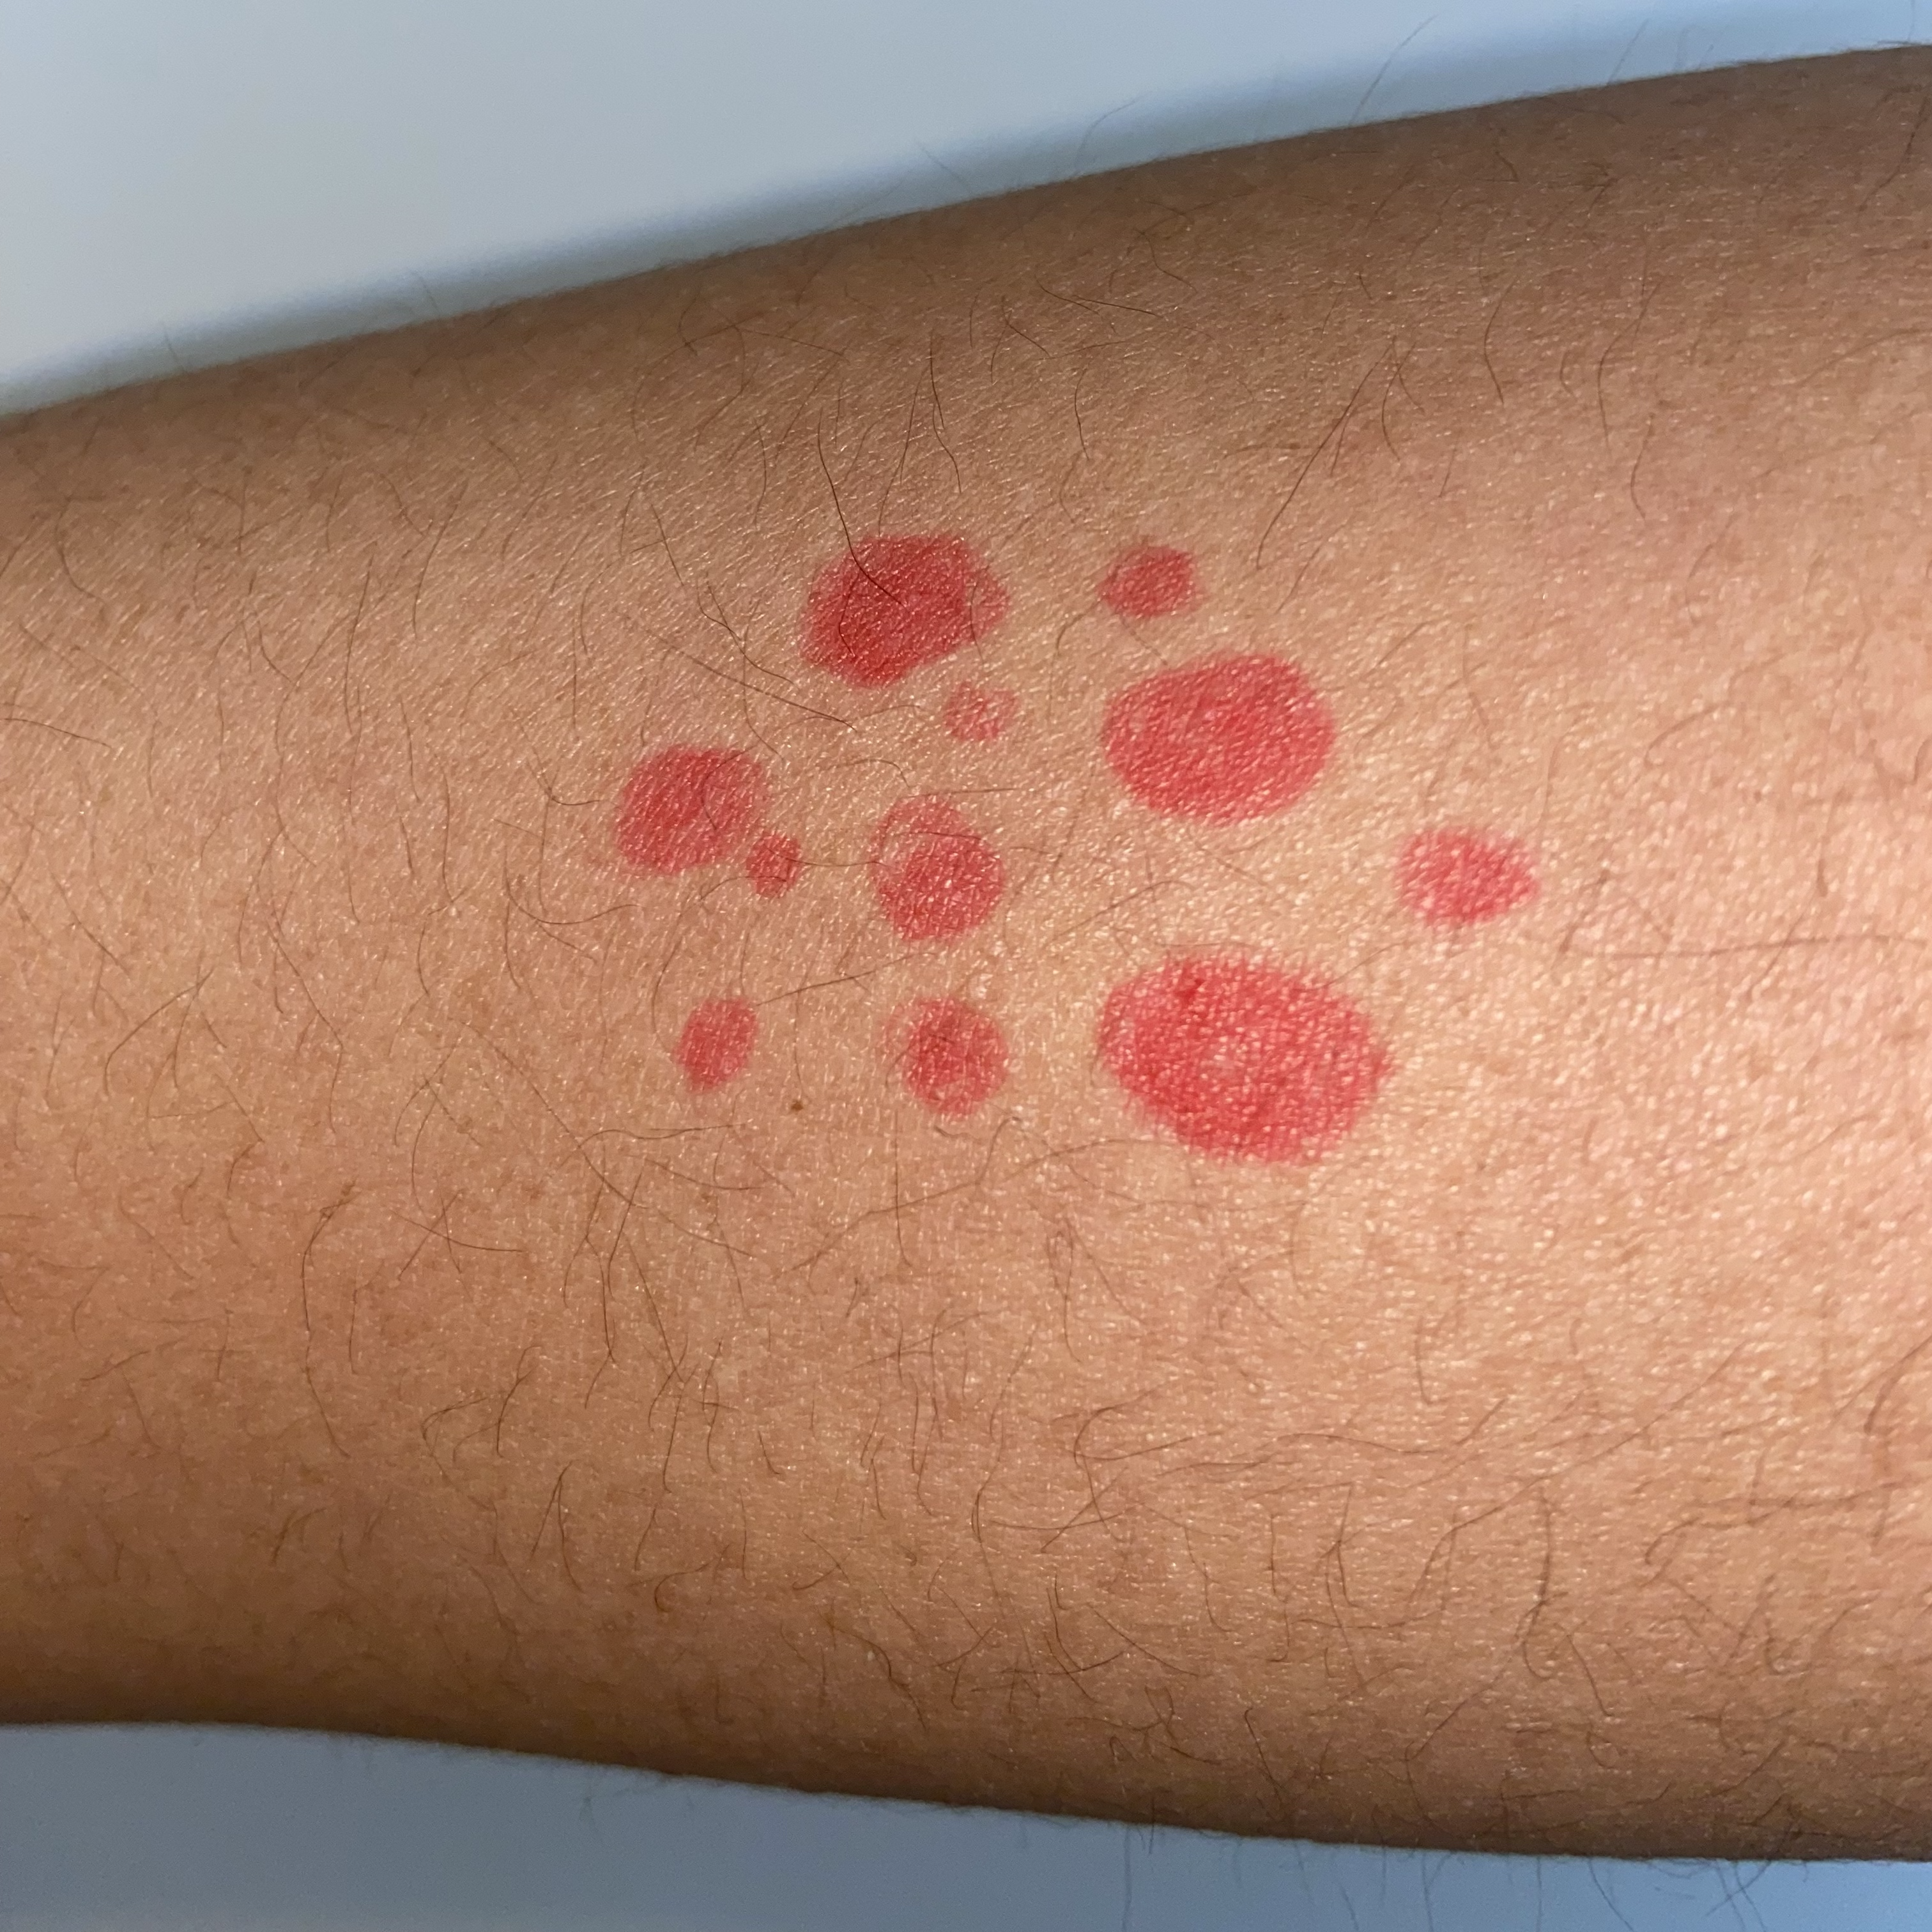
\includegraphics[width=\textwidth]{img/Reference.jpg}
        \caption{Good Quality}
    \end{subfigure}
    \hfill
    \begin{subfigure}[b]{0.24\textwidth}
        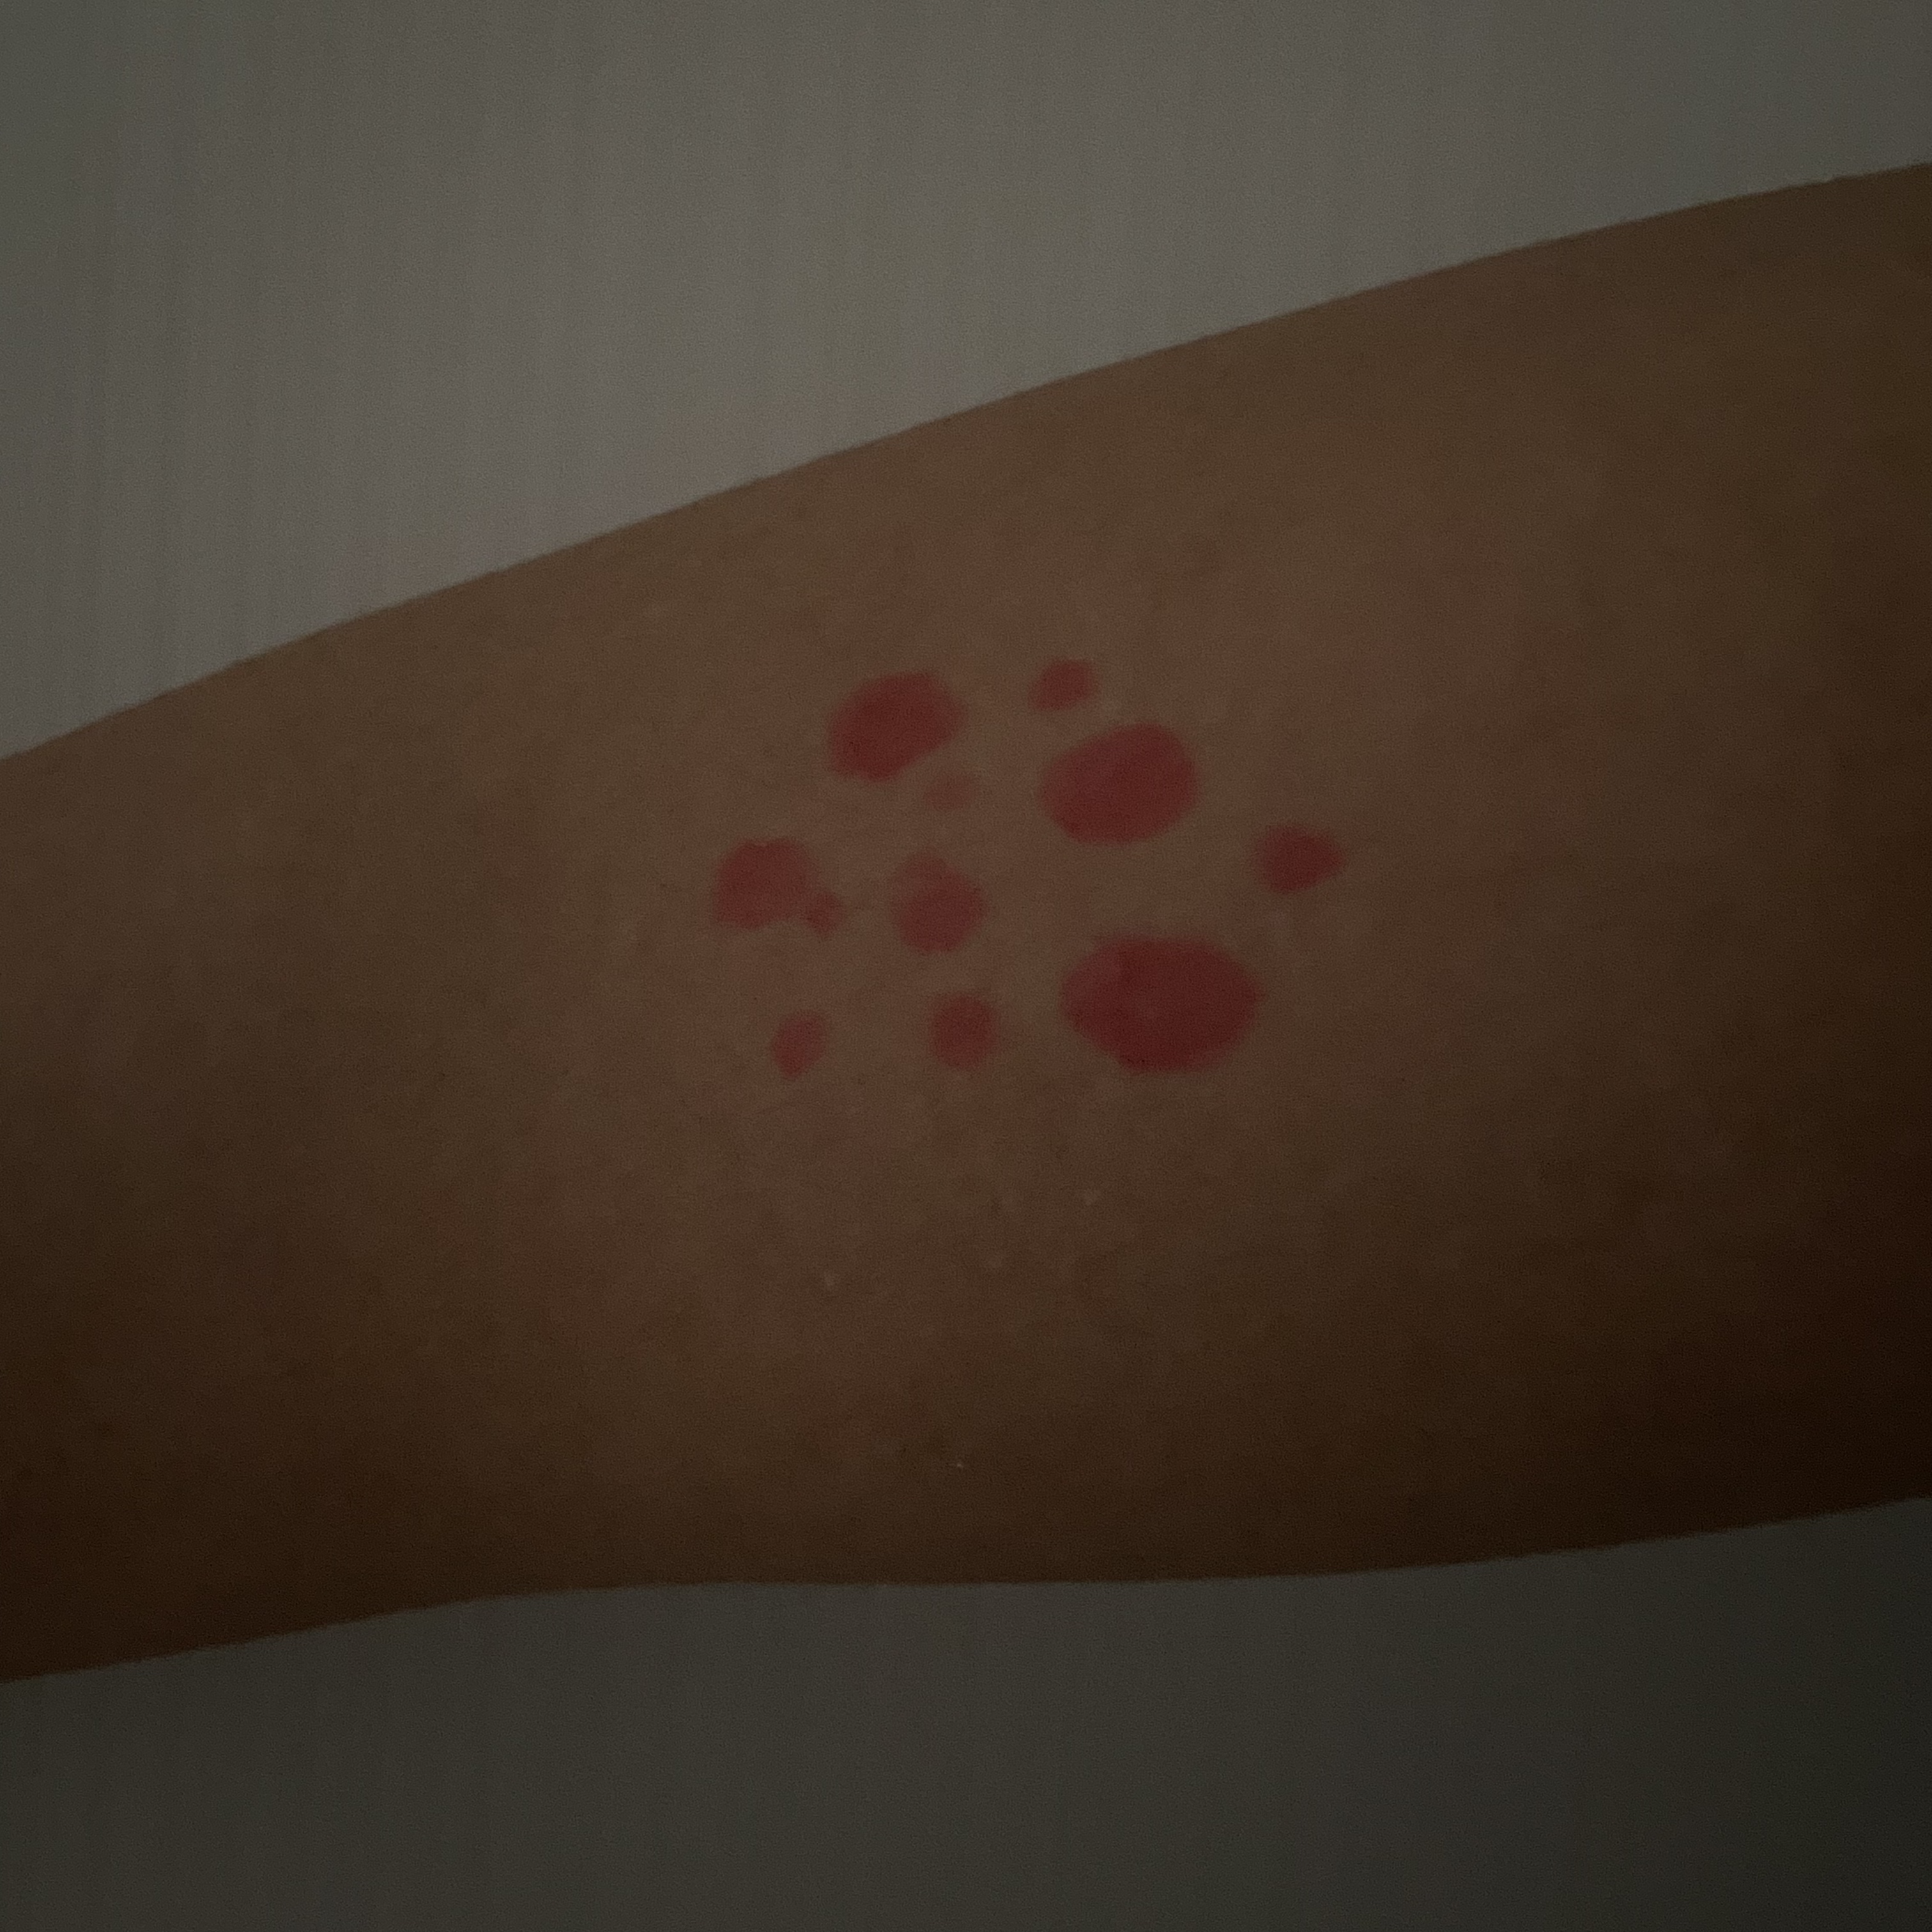
\includegraphics[width=\textwidth]{img/Lighting.jpg}
        \caption{Lighting}
        \label{fig:lighting}
    \end{subfigure}
    \hfill
    \begin{subfigure}[b]{0.24\textwidth}
        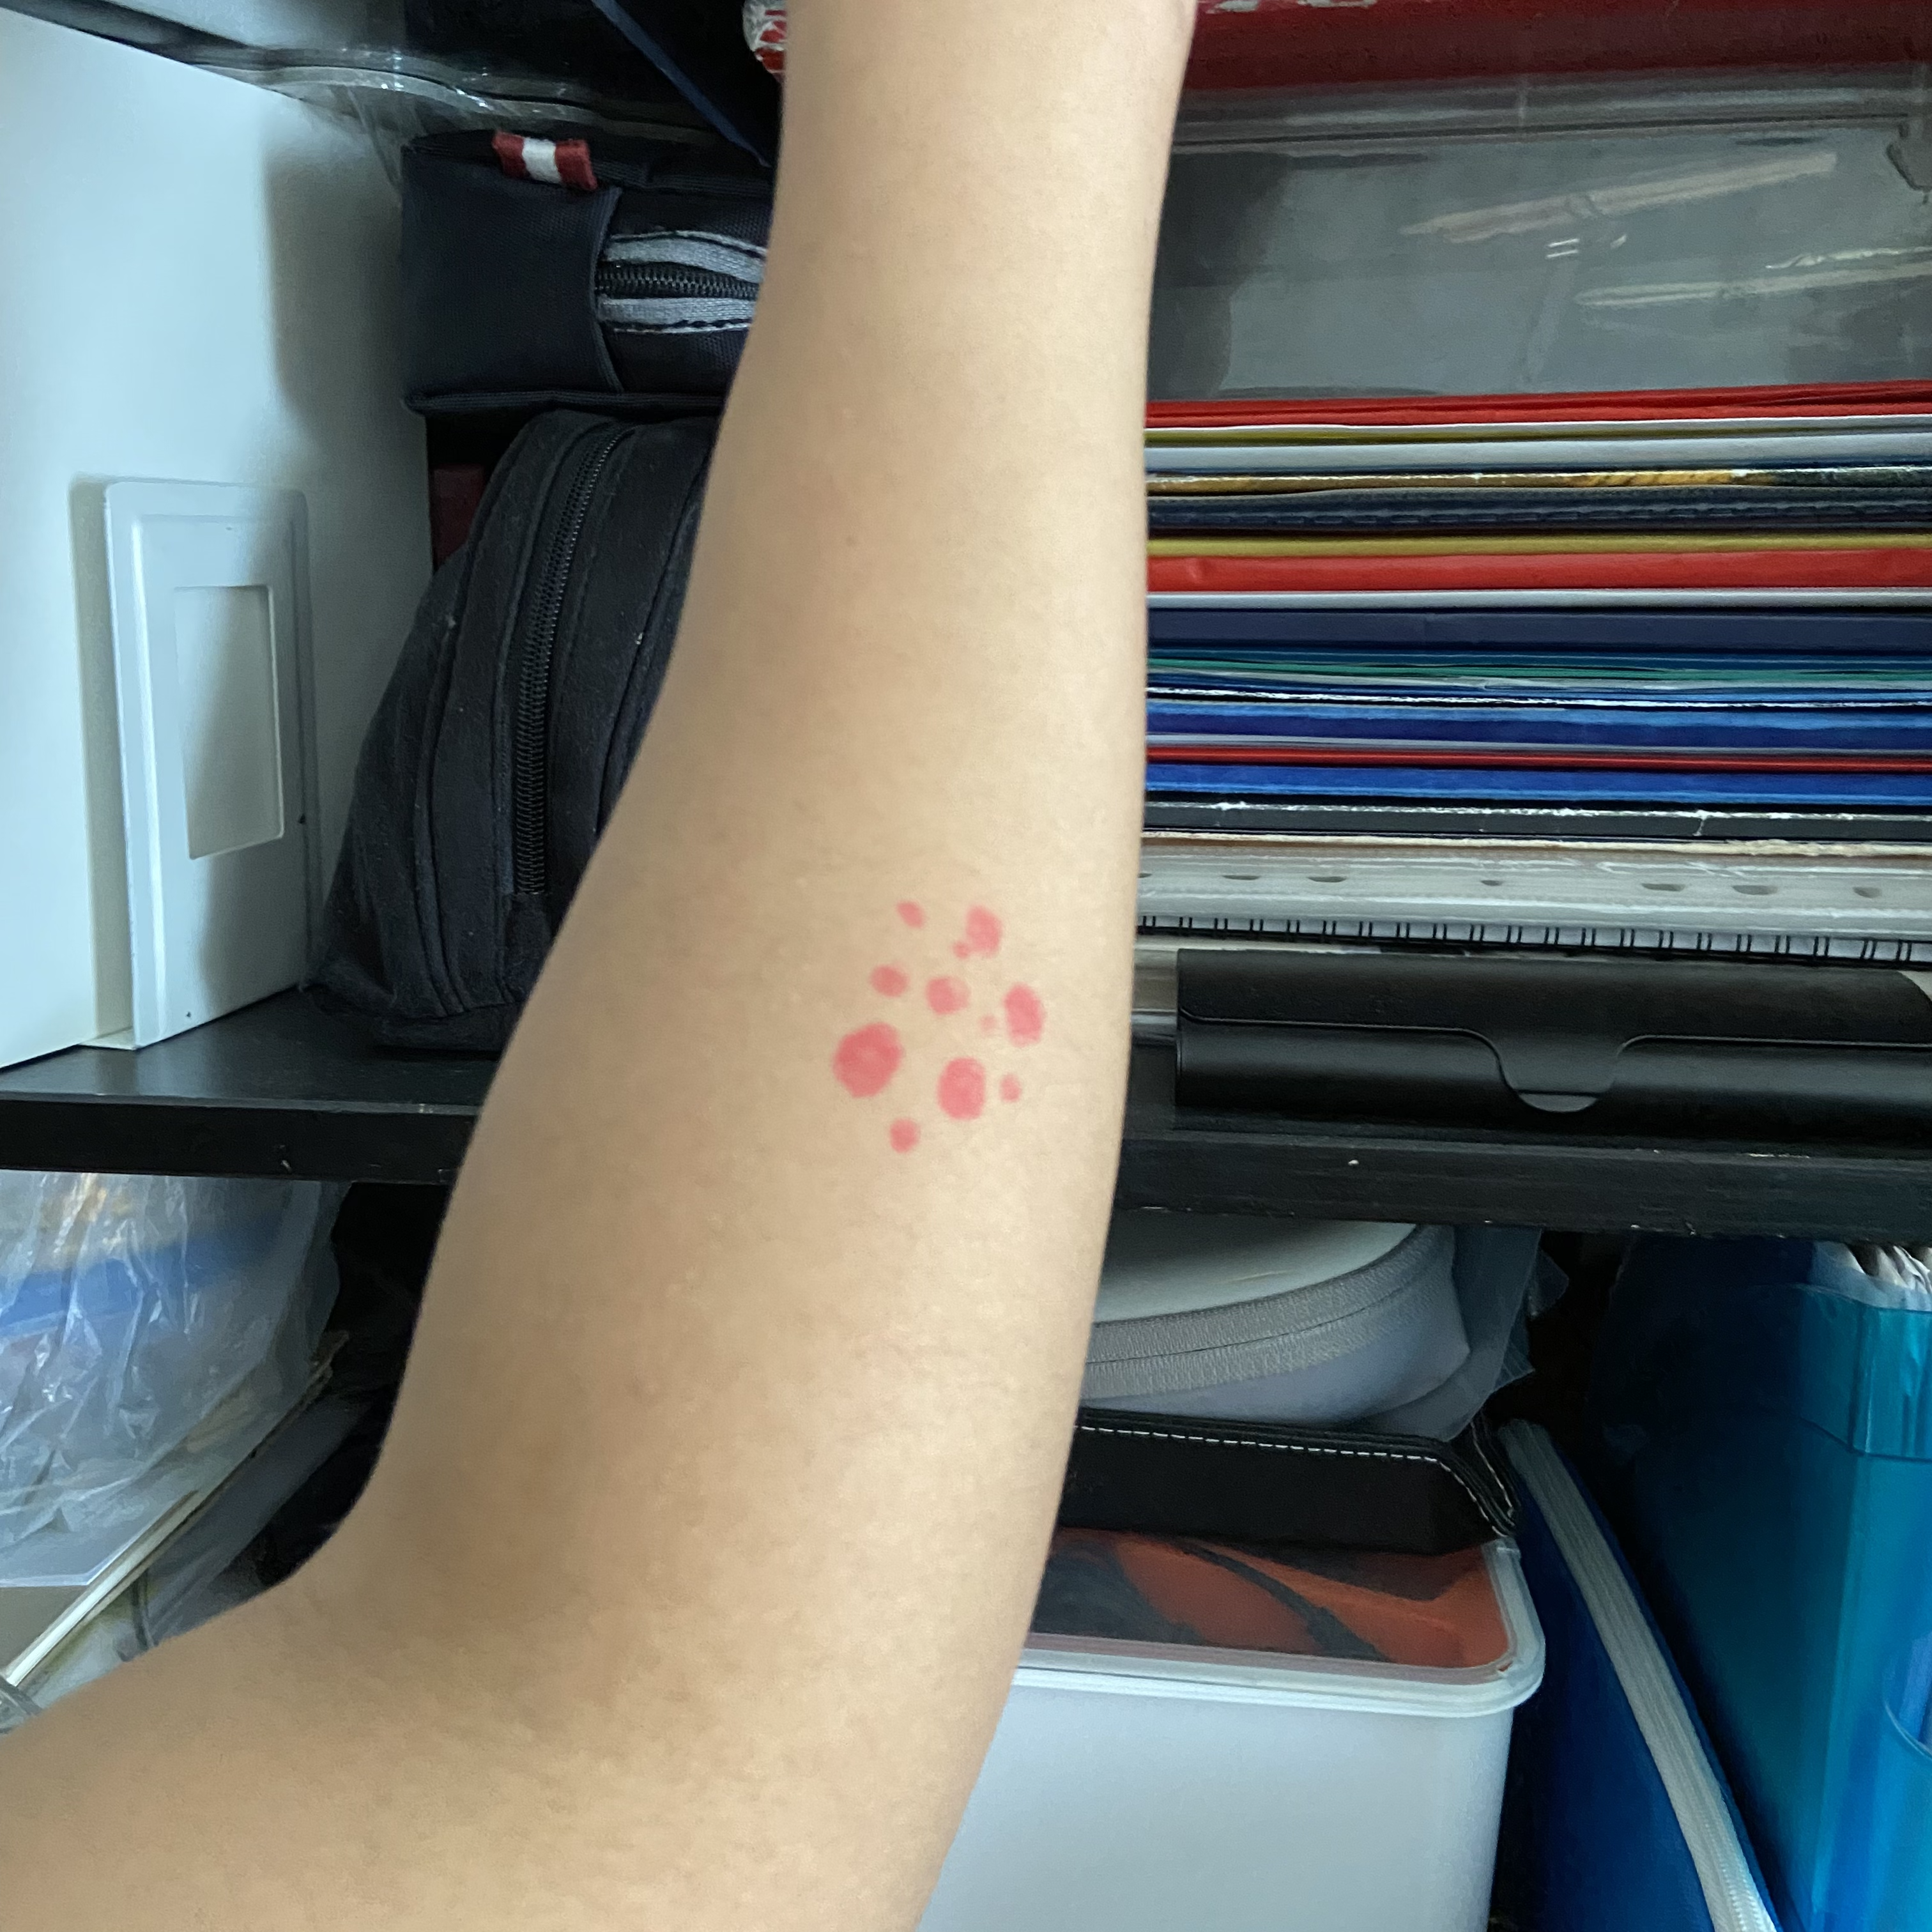
\includegraphics[width=\textwidth]{img/Background.jpg}
        \caption{Background}
        \label{fig:background}
    \end{subfigure}
    \hfill
    \begin{subfigure}[b]{0.24\textwidth}
        \includegraphics[width=\textwidth]{img/FoV.jpg}
        \caption{Field of View}
        \label{fig:FoV}
    \end{subfigure} 

    \begin{subfigure}[b]{0.24\textwidth}
        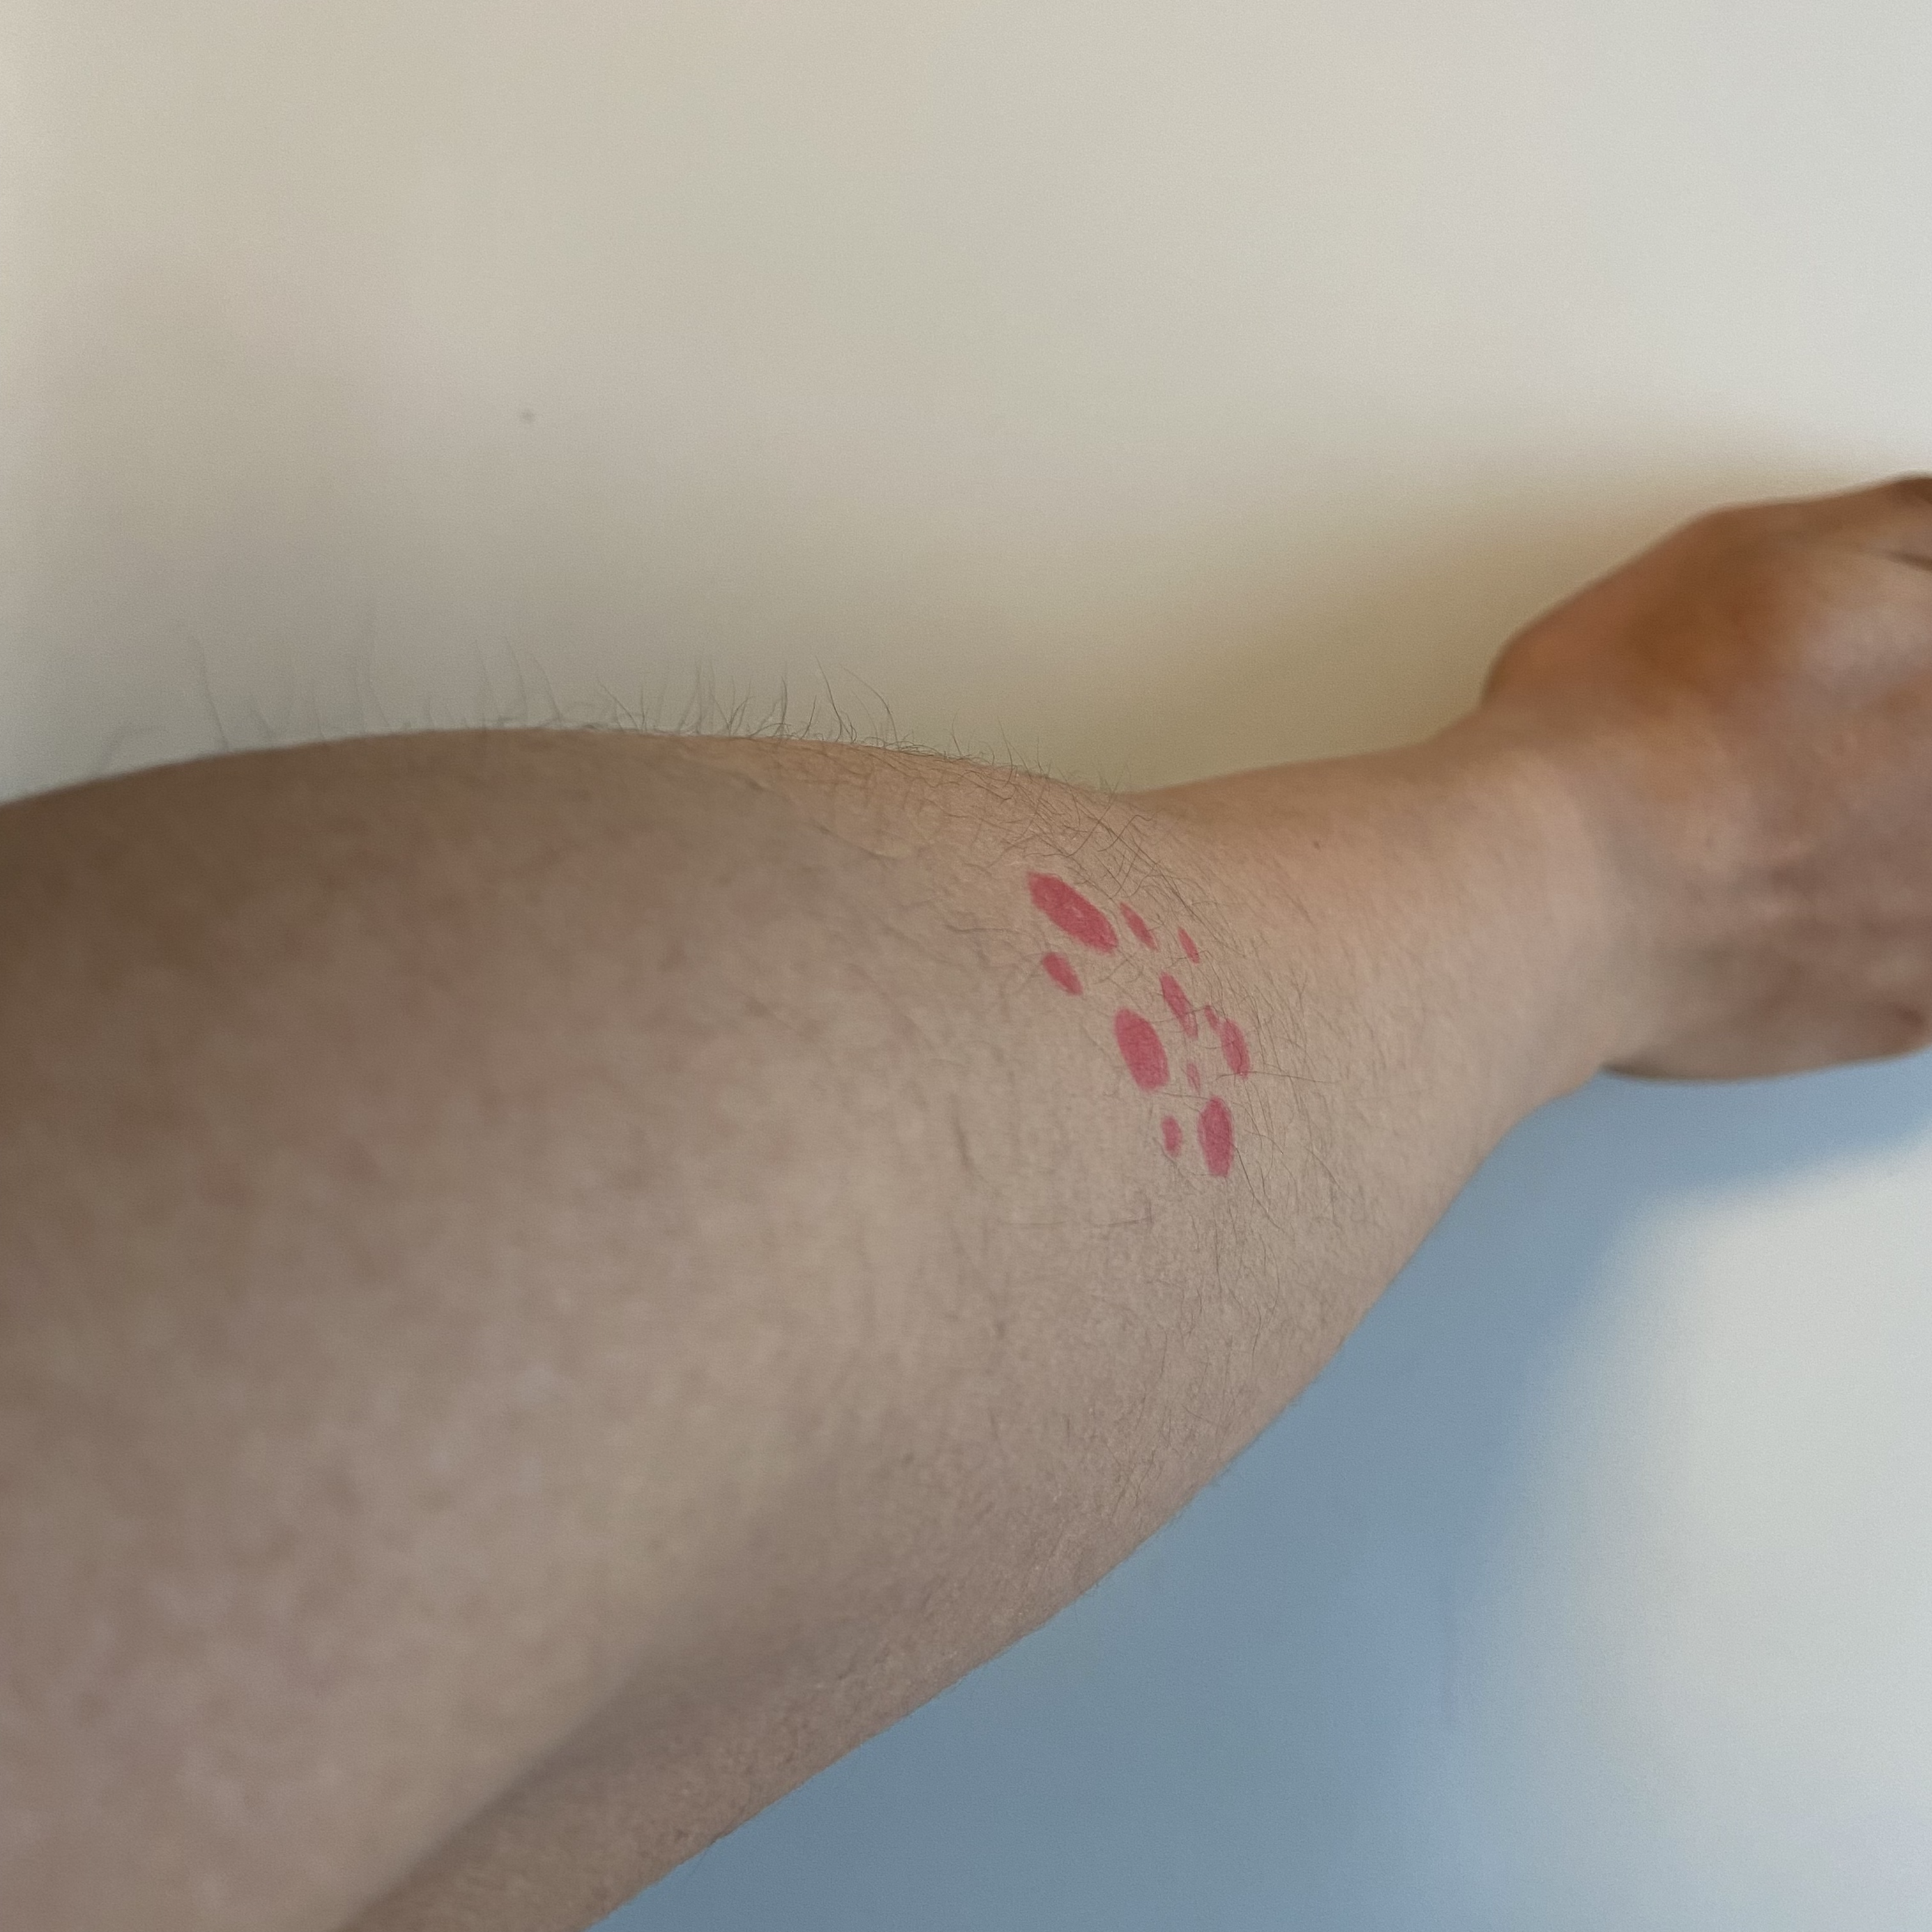
\includegraphics[width=\textwidth]{img/Orientation.jpg}
        \caption{Orientation}
        \label{fig:orientation}
    \end{subfigure}
    \hfill
    \begin{subfigure}[b]{0.24\textwidth}
        \includegraphics[width=\textwidth]{img/Focus.jpg}
        \caption{Focus}
        \label{fig:focus}
    \end{subfigure}
    \hfill
    \begin{subfigure}[b]{0.24\textwidth}
        \includegraphics[width=\textwidth]{img/Resolution.jpg}
        \caption{Resolution}
        \label{fig:resol}
    \end{subfigure}
    \hfill
    \begin{subfigure}[b]{0.24\textwidth}
        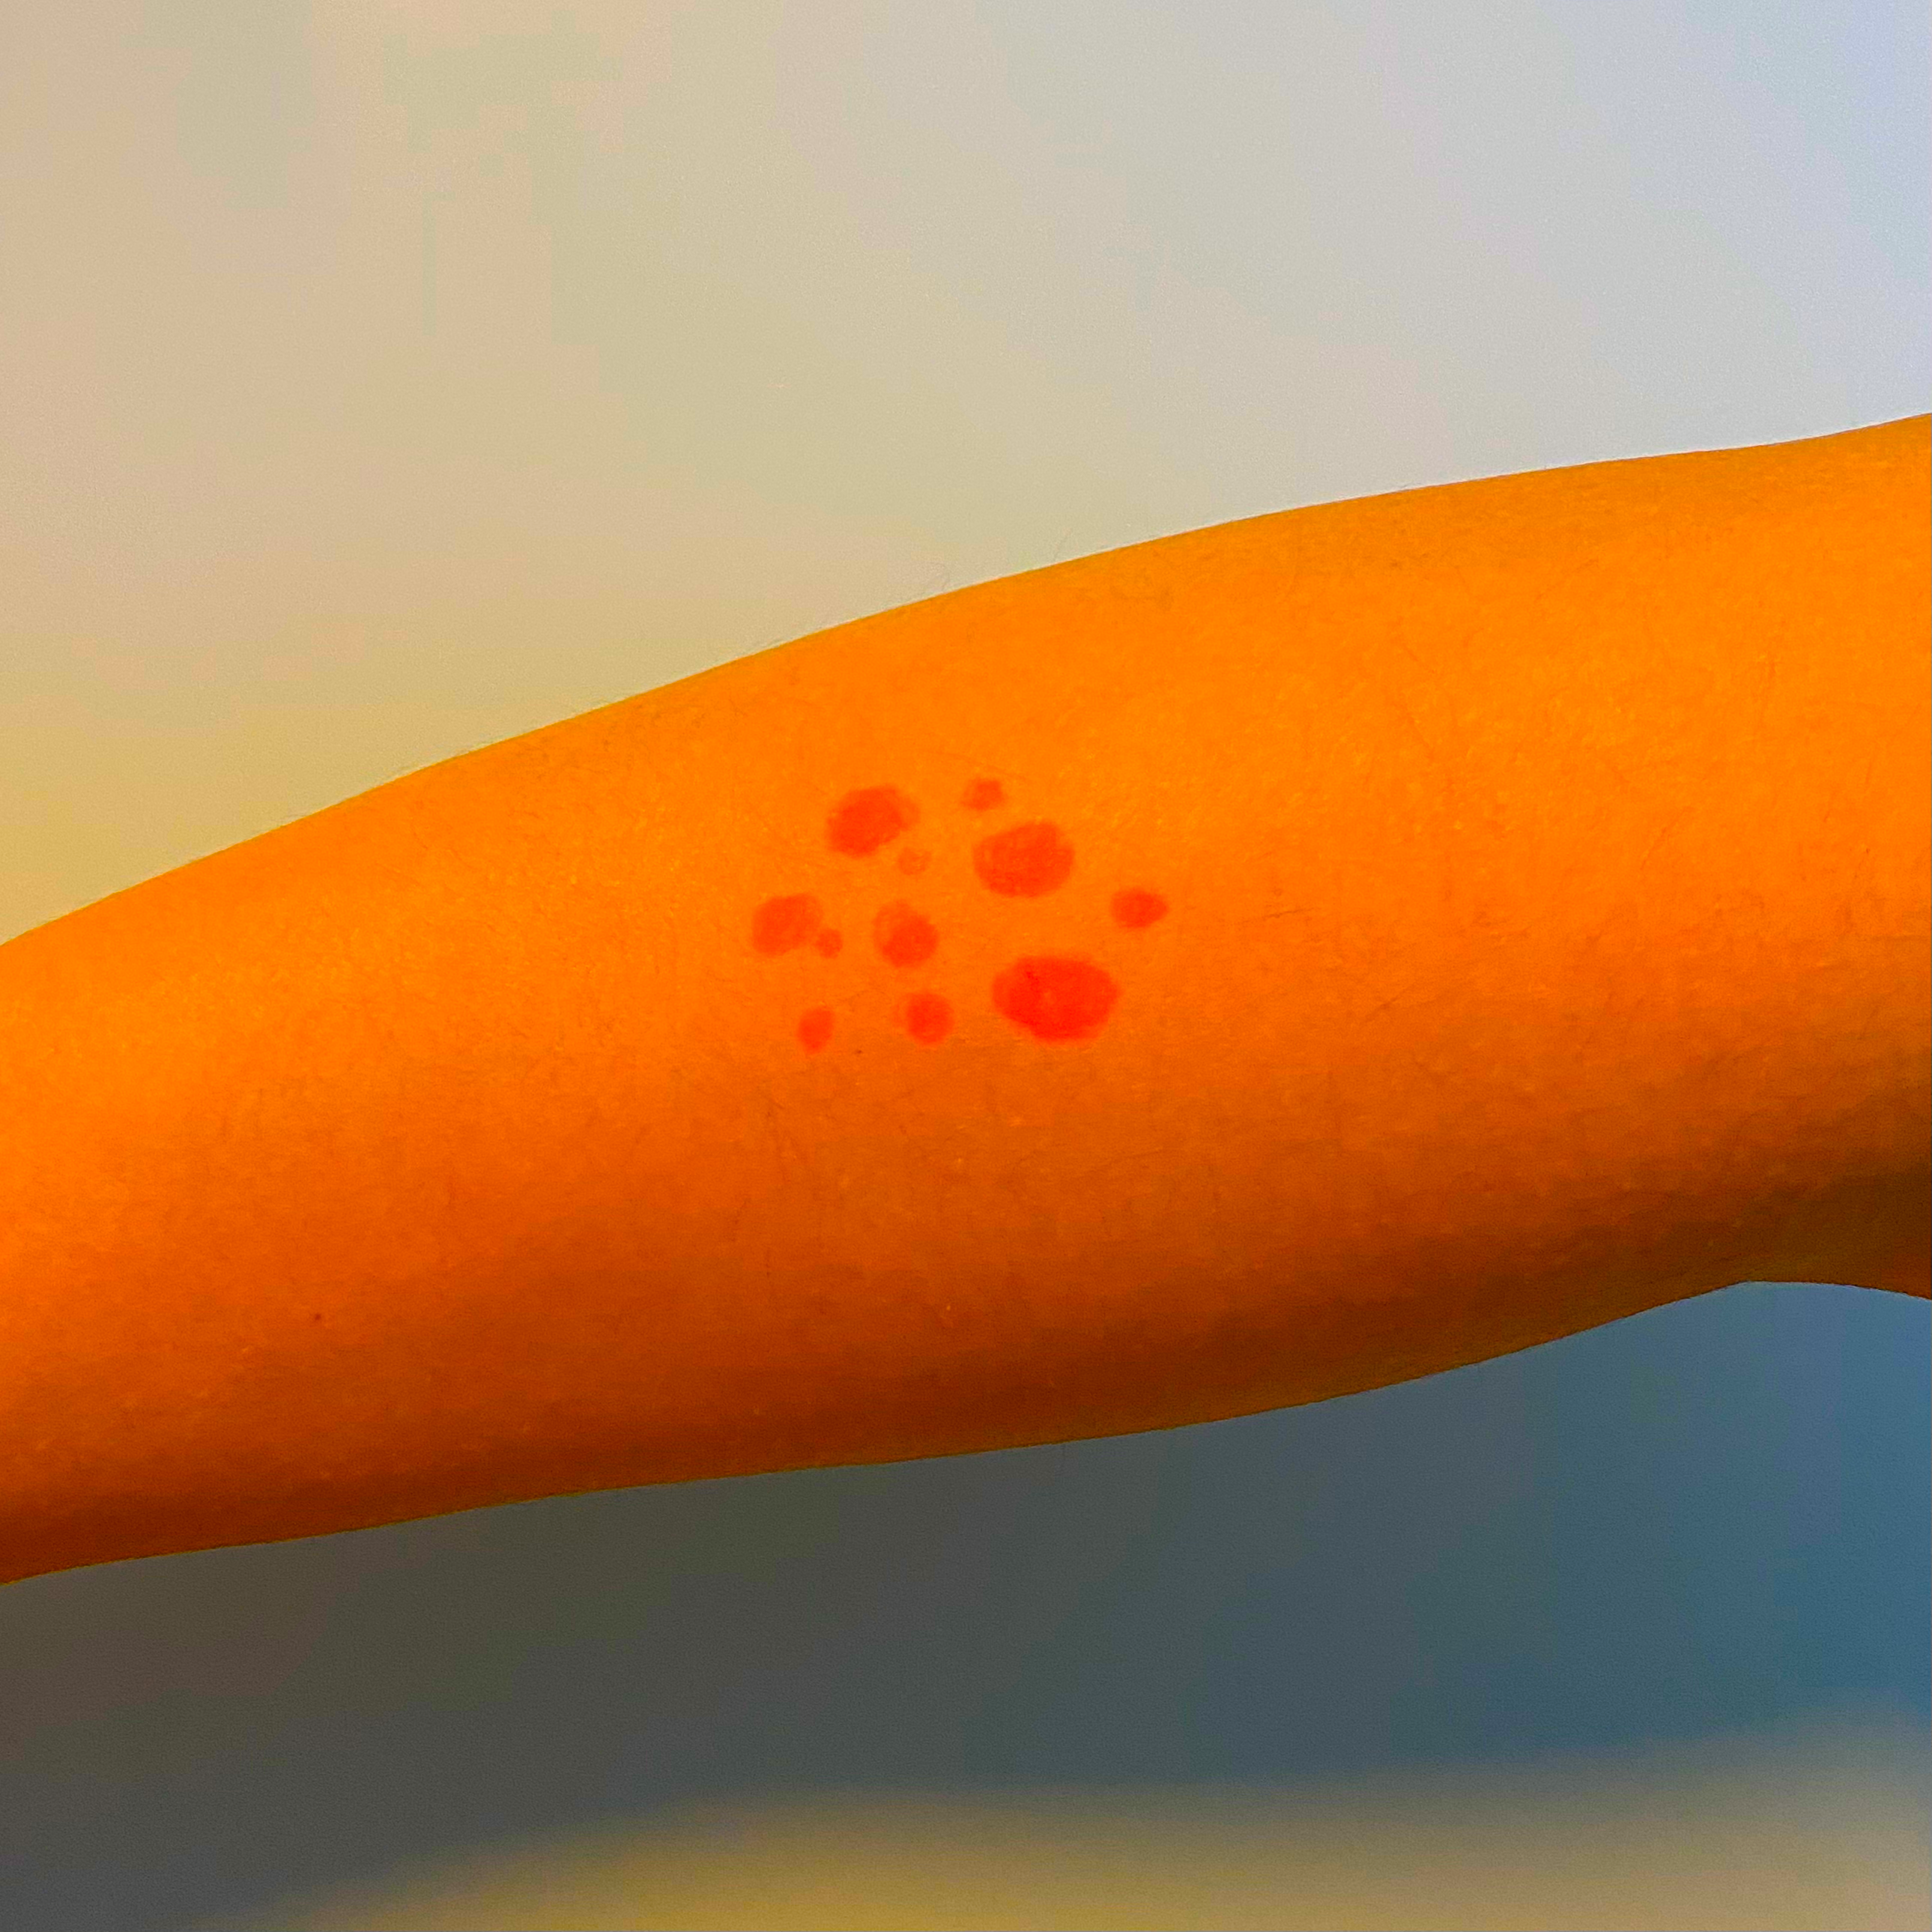
\includegraphics[width=\textwidth]{img/Color.jpg}
        \caption{Color Calibration}
        \label{fig:cc}
    \end{subfigure}
    \caption{Example images illustrating common distortions used in Teledermatology Image Quality Assessment. (Created by the Author)}
    \label{fig:quality_criteria}
\end{figure}
\begin{enumerate}
    \item \textbf{Lighting}:  Adequate illumination is critical. It should be even and diffuse, avoiding harsh shadows or overexposure that could obscure skin lesions or lead to misinterpretation of the skin's condition. \textbf{Remark} Position the light source evenly to avoid shadows and overexposure. Natural light or diffused artificial light can help illuminate the skin lesion uniformly and reduce glare.
    \item \textbf{Background}: A neutral and uncluttered background helps to focus attention on the dermatological issue without distraction, ensuring that the skin lesion is the most prominent feature in the image. \textbf{Remark} Use a plain, non-reflective background to minimize distractions and ensure the focus remains on the skin lesion. A neutral-colored backdrop, such as white or gray, is ideal for providing contrast with the lesion.
    \item \textbf{Field of View}: The image should be framed to include a clear view of the lesion as well as sufficient surrounding area to provide context, which can be crucial for accurate diagnosis. \textbf{Remark} Center the skin lesion or area of interest within the frame to ensure complete coverage and avoid cutting off important details. Maintain a consistent distance between the camera and the skin to prevent distortion.
    \item \textbf{Orientation}: Proper orientation of the image is vital. It should align with standard anatomical positions, allowing the dermatologist to easily interpret the image in relation to the patient's body. \textbf{Remark} Orient the camera perpendicular to the skin surface to capture images in the correct orientation. Align the camera with the skin lesion to maintain consistency and facilitate accurate comparison between images.
    \item \textbf{Focus \& Depth of Field}: Sharp focus on the lesion is a necessity, with a depth of field that keeps the entire area of interest in clear detail, as blurring can mask important characteristics of skin conditions. \textbf{Remark} Ensure the camera is in focus and adjust the aperture to achieve sufficient depth of field. Focus on the skin lesion to capture sharp, detailed images without blurriness or loss of clarity.
    \item \textbf{Resolution}: The image must be high resolution to reveal fine details of the skin. A higher pixel count can facilitate a more thorough examination and better clinical decision-making. \textbf{Remark} Use a camera with high-resolution capabilities to capture fine details and nuances of the skin lesion. Adjust the camera settings to the highest resolution possible to ensure clarity and precision in the image.
    \item \textbf{Color Calibration}:  Accurate color reproduction is necessary for the assessment of skin lesions. Any color distortion can lead to misdiagnosis, especially in conditions where hue is a diagnostic clue. \textbf{Remark} Calibrate the camera settings to accurately reproduce colors and skin tones. Avoid harsh lighting or color casts that may distort the color representation of the skin lesion. Use a color reference chart or white balance settings to ensure color accuracy.
\end{enumerate}
Each of these quality criteria contributes to the diagnostic accuracy in teledermatology by ensuring that the images convey the true nature of the skin condition. Just as in traditional dermatology, where the dermatologist's visual assessment is a key diagnostic tool, in teledermatology, the image serves as the eyes of the dermatologist. Therefore, optimizing these criteria is crucial to the successful application of teledermatology services.


\subsection{Teledermatology Datasets}
\label{sub:DatasetsTD}
The following datasets are valuable resources for teledermatology research and applications, especially notable for their accessibility and diversity. These datasets are not strictly confined to clinical settings or dermoscopic images and include patient-taken images, making them highly relevant for practical teledermatology purposes where clinical settings may vary:
\begin{itemize}
    \item \textbf{ACNE04}: This dataset focuses on acne severity and lesion counting, containing 1,457 images with detailed annotations for training and testing purposes \autocite{ACNE04}.
    \item \textbf{DDI}: Provides 656 high-quality images curated by dermatologists for detailed skin tone evaluation and diagnostic accuracy \autocite{DDI}.
    \item \textbf{Derm7pt}: Utilizes 1,011 lesion cases to train a neural network for classifying skin lesions and melanoma using the 7-point checklist \autocite{Derm7pt}.
    \item \textbf{Fitzpatrick17k}: Includes 16,577 images annotated for Fitzpatrick skin type across 114 different skin conditions \autocite{F17K}.
    \item \textbf{Monkeypox Dataset 2022}: Contains approximately 1,905 images focused on monkeypox, useful for developing diagnostic tools \autocite{Monkeypox}.
    \item \textbf{PAD-UFES-20}: Comprises 2,298 clinical images from smartphones, enriched with clinical metadata for comprehensive research \autocite{PAD-UFES-20}.
    \item \textbf{SCIN}: Emerged from a crowdsourcing initiative, this dataset contains 10,408 images capturing a broad spectrum of dermatological conditions \autocite{SCIN}.
\end{itemize}
\vspace{\baselineskip}
\noindent
These datasets collectively contribute to the advancement of teledermatology by providing varied, real-world data crucial for developing effective diagnostic tools and algorithms. \par 

\subsection{Approaches to Image Quality Assessment in Teledermatology}
\label{sub:ApproachesIQAinTeledermatology}
To understand the various approaches to Image Quality Assessment (IQA) within teledermatology, it is instructive to review related works that have contributed to the field. These studies not only offer insights into the methodologies employed for assessing image quality but also highlight the specific image distortions that are often targeted. Furthermore, by examining the architectures of the algorithms and the criteria used to classify image quality, we can discern the strengths and weaknesses of each approach. \par

\subsubsection{TrueImage: A Machine Learning Algorithm to Improve the Quality of Telehealth Photos}
\label{subsub:TrueImage}
The TrueImage algorithm prioritizes real-time, interactive feedback for patients taking dermatological images via their smartphones. Its three-stage process includes semantic segmentation to identify skin regions, feature generation focusing on blur, lighting, and zoom, and logistic regression classifiers that predict image quality and specific reasons for poor quality \autocite{TrueImage}. \par
\vspace{\baselineskip}
\noindent
The prototype exhibits promise, demonstrating the capability to reject approximately half of sub-par quality images while retaining around 80\% of good quality images. This suggests its potential utility in a clinical setting, where it could save time for both clinicians and patients by pre-screening image quality and offering specific feedback to improve poor submissions \autocite{TrueImage}.
\par
\vspace{\baselineskip}
\noindent
Yet, TrueImage’s current limitation lies in its modest dataset and the training data's lack of diversity regarding skin types, which could lead to biased quality assessments. Furthermore, while the algorithm excels at detecting blurriness, it is less effective at assessing lighting conditions and zoom, which are critical factors in teledermatology \autocite{TrueImage}.\par

\subsubsection{ImageQX: Explainable Image Quality Assessments in Teledermatological Photography}
\label{subsub:ImageQX}
ImageQX offers an automated, deployable method for IQA in teledermatology, addressing common image distortions: such as poor framing, bad lighting, blur, low resolution, and distance issues. With an architecture that employs the EfficientNet-B0 as a lightweight feature extractor. The network then employs linear layers, batch normalization, and dropout layers to predict poor image quality reasons, integrating them to forecast overall image quality \autocite{ImageQX}.
\par
\vspace{\baselineskip}
\noindent
The approach is data-driven, validated on a substantial dataset annotated by dermatologists, which underscores its potential for real-world applicability. With a macro F1-score of 0.73 for image quality assessment, ImageQX demonstrates expertise comparable to dermatologists and a capability for explainability via attention maps that can guide patients to retake pictures more effectively \autocite{ImageQX}.
\par
\vspace{\baselineskip}
\noindent
However, while ImageQX achieves high specificity, suggesting minimal disruption to patient experience by incorrectly rejecting high-quality images, its predictive performance for certain poor quality explanations like 'bad framing' remains low, with an F1-score of 0.37 \autocite{ImageQX}. This indicates room for improvement in addressing certain types of distortions, though the network’s size (15MB) makes it an attractive option for mobile deployment.
\par
\vspace{\baselineskip}
\vspace{\baselineskip}
\noindent
ImageQX stands out with its deep learning approach that uses a convolutional neural network (CNN) trained on a dataset of images labeled for quality by board-certified dermatologists. The network architecture is based on the lightweight EfficientNet-B0, which facilitates deployment on mobile devices. This model's training utilized a large dataset of 36,509 images, where the photographs were annotated for common quality issues, such as framing, lighting, blur, resolution, and distance from the subject.
\par
\vspace{\baselineskip}
\noindent
The strength of ImageQX lies in its explainability and its ability to provide reasons for poor image quality, aligning closely with the common distortions identified by dermatologists. It achieves a high macro F1-score, suggesting that its performance in image quality assessment is on par with expert human raters. However, some limitations include the difficulty of explaining certain quality issues like 'blurry' images, which had lower inter-rater agreement scores. The model's reliance on dermatologist-annotated images also points to the importance of the quality and diversity of the training dataset for its generalizability and accuracy. \par
\vspace{\baselineskip}
\noindent
In conclusion, both ImageQX and TrueImage present pioneering steps towards automated IQA in teledermatology, each with strengths such as deployability and real-time feedback capabilities. Their current challenges include the need for more diverse training data, improved detection of certain distortions, and further validation in real-world settings. Addressing these challenges will be crucial for their successful integration into teledermatological practices, ultimately contributing to more efficient and effective remote dermatological care. \par

\subsection{Challenges and Opportunities in Teledermatology}
\label{sub:ChallengesOpportunitiesTeledermatology}
Teledermatology has fundamentally changed how dermatological care is accessed, particularly in remote or underserved areas. However, the field faces several challenges that intersect with the focus of this thesis on image quality assessment.\par
\vspace{\baselineskip}
\noindent
One major challenge is the variability in image quality, which stems from patients using a wide range of devices in uncontrolled environments to capture images. This variability can severely impact the consistency and reliability of diagnoses made remotely. Additionally, technological barriers such as disparities in access to high-quality digital devices and varying levels of digital literacy among patients can further affect the quality of submitted images. Moreover, ensuring the privacy and security of sensitive dermatological images transmitted over the internet remains a critical concern that needs continuous attention to safeguard patient data.\par
\vspace{\baselineskip}
\noindent
On the opportunity front, recent advancements in image processing and machine learning technologies present significant potential to automatically enhance image quality and correct common distortions. This can greatly aid in improving diagnostic accuracy and efficiency. There is also a considerable opportunity to develop and implement standardized guidelines for image capture in teledermatology. Such standardization can help minimize quality variability and streamline the diagnostic process. Furthermore, the integration of artificial intelligence to provide real-time feedback to patients on improving image quality can enhance the effectiveness of teledermatology services by ensuring that only high-quality images are evaluated by dermatologists.\par
\vspace{\baselineskip}
\noindent
By tackling these challenges and leveraging the emerging opportunities, teledermatology can continue to evolve and play a crucial role in modern healthcare, enhancing access and efficiency in dermatological care across diverse populations.\par

\chapter{Methodology}
\label{ch:Methodology}
Based on the insights from \autoref{ch:LiteratureReview}, this chapter provides an overview of the key ideas and concepts needed to achieve the research goals. The following sections will explore important concepts related to image quality assessment in teledermatology and explain the reasoning behind this work. Detailed implementation of these steps will be covered in \autoref{ch:Implementation}.\par

\section{Explorative Approach}
\label{sec:ExplorativeApproach}
\begin{figure}[ht]
    \centering
    \includegraphics[keepaspectratio,width=13cm]{img/DecisionCycle.jpg}
    \caption{Illustration of the explorative approach, including the stages of initialization, idea generation, idea selection, and implementation. The lower part of the figure shows the decision cycles \autocite{DesignThinking}.}
    \label{fig:decision_cycle}
\end{figure}
\noindent
Teledermatology, especially when focused on Image Quality Assessment (IQA), offers many opportunities for innovation due to the different types of image distortions and ways to address them. To handle this complexity, an exploratory approach was used in this research. This approach is flexible and innovative, allowing for adjustments as new information is discovered, unlike traditional methods like the waterfall approach. \par
\vspace{\baselineskip}
\noindent
At the beginning, the problem was broadly defined, allowing for a flexible and adaptive approach. The research progressed through creative problem-solving with multiple learning cycles, refining ideas and methods iteratively. The project was divided into two main phases. In the \textit{Diverging Phase}, the research question’s scope was expanded to generate new ideas continuously, based on insights from the ongoing literature review. In the \textit{Converging Phase}, the focus on combining these ideas into clear findings and conclusions, aiming to create a unified understanding of the initial problem. This exploratory model is shown in \autoref{fig:decision_cycle}, which illustrates the stages of starting, generating ideas, selecting ideas, and implementation, along with the decision cycles \autocite{DesignThinking}.

\section{Project Control}
\label{sec:ProjectMonitoring}
Even with an exploratory approach, it is important to have a rough timeline to guide the research tasks. A workflow was established before starting, detailed in the planning document attached to this thesis. \par
\noindent
There are three key milestones identified in the first half of the project, each crucial for its success: \par
\vspace{\baselineskip}
\noindent
\textbf{Understanding Teledermatology}: Gaining a thorough understanding of the field to ensure all subsequent actions are relevant and well-informed. \par
\vspace{\baselineskip}
\noindent
\textbf{State of the Art in IQA}: Identifying the latest developments in IQA to ensure the methods used are up-to-date and effective. \par
\vspace{\baselineskip}
\noindent
\textbf{Availability of Teledermatology Data}:  Securing access to appropriate datasets for conducting meaningful IQA. \par
\vspace{\baselineskip}
\noindent
These milestones are essential because each phase of the project relies on the successful completion of the previous one. Missing any of these milestones could significantly impact the project and might require a fundamental reassessment of the objectives outlined in \autoref{sec:Objectives}. \par

\section{Research Steps}
\label{sec:ResearchSteps}
As mentioned, this study was exploratory, so it was not possible to follow a strict, step-by-step process. However, for the individual key steps, I took a systematic approach to stay organized and ensure that each step was done in the right order: \par

\subsection{Literature Review}
\label{sub:LR}
First, I began by getting an overview of my research field. As I was new to the domain of teledermatology and dermatology, this initial step was crucial. By researching and reading relevant literature, I gradually built a solid understanding of the field. Next, I identified the core topics related to my research objectives. Once I had these key topics, I carefully selected the databases to search, focusing on those most relevant to my field: PubMed\footnote{https://pubmed.ncbi.nlm.nih.gov}, Google Scholar\footnote{https://scholar.google.com}, IEEE Xplore\footnote{https://ieeexplore.ieee.org/Xplore/home.jsp}, Connected Papers\footnote{https://www.connectedpapers.com}, and Papers with Code\footnote{https://paperswithcode.com}. Using these databases, I applied search filters to narrow down the results, such as limiting the search to articles published after 2020. \par
\vspace{\baselineskip}
\noindent
I reviewed the titles of the search results and opened the ones that seemed interesting. After that, I read the abstracts to determine their relevance. Depending on the relevance of the abstract and some of the figures, I decided whether to read the full paper. Additionally, for state-of-the-art methods, I focused on finding and reading papers that had published their code and model weights if models were trained. This systematic approach ensured that my literature review was thorough and focused on the most relevant and up-to-date research. \par

\subsection{Data Collection and Preparation}
\label{sub:DataCollection}
In searching for a suitable dataset to evaluate image quality in teledermatology, a major challenge was the lack of Mean Opinion Score (MOS) or Differential Mean Opinion Score (DMOS) in teledermatology datasets, as commonly found in traditional IQA datasets mentioned in \autoref{sub:BenchmarkDatasetsIQA}. This scarcity is due to the resource-intensive nature of labeling images in the medical field. \par
\vspace{\baselineskip}
\noindent
To address this gap, I created a distortion pipeline that synthetically distorts images based on the seven criteria defined in \autoref{sub:QualityCriteriaTeledermatology}. Each type of distortion has five levels of severity, with the severity indicating how poor the image quality is. These distortions are carefully selected to simulate real-world imperfections commonly encountered in teledermatology. Each image is then labeled according to the severity and type of distortion applied, creating a dataset that not only includes the distorted images but also features precise annotations regarding their quality. This allowed me to artificially create labels for my images. For this, I needed high-quality images to start with. I chose two datasets: the SCIN dataset for its relevance and uniqueness, and the Fitzpatrick17k dataset to complement the SCIN dataset. \par
\vspace{\baselineskip}
\noindent
Unlike many dermatology datasets that mainly focus on skin cancer diagnostics by classifying malignant and benign tumors, the SCIN dataset covers a broader range of common dermatological conditions, including allergic, inflammatory, and infectious diseases. These conditions are frequently encountered in everyday clinical practice but are underrepresented in existing datasets. The SCIN dataset is particularly valuable because it captures images of early-stage conditions. Over half of the images were taken less than a week from the onset of symptoms, with 30\% captured less than a day after symptoms appeared \autocite{SCIN}. These are conditions patients are likely to consult via teledermatology platforms before visiting traditional healthcare settings. The Fitzpatrick17k dataset contains more clinical setting images, which provide good quality but do not represent the variability seen in typical teledermatology images \autocite{F17K}, so I used the Fitzpatrick17k dataset only for training purposes. In total, I filtered 475 good quality images from the Fitzpatrick17k dataset and another 475 good quality images from the SCIN dataset, along with 200 randomly selected test images from the SCIN dataset.\par
\vspace{\baselineskip}
\noindent
This approach to dataset preparation not only tailored the data to the specific needs of this research but also established a framework for systematically assessing image quality in teledermatology. This preparation is crucial for the next phases of the project, which involve training and validating the image quality assessment model to ensure it can reliably perform in real-world teledermatology applications. \par

\subsection{Feature Extraction}
\label{sub:FeatureExtraction}
Feature extraction is the next important step where the SimCLR model from ARNIQA is used to identify key features from the distorted images. These features capture the patterns of distortions that affect image quality. The extracted features and the generated labels are then used to train different models, including XGBoost regressor, XGBoost classifier, and MLP regressor, to see which one works best for assessing image quality. \par

\subsection{Training and Validation}
\label{sub:TrainVal}
The training of the models is based on the prepared training data. Since I am generating labels and distorted images, I am not restricted by the original amount of data. I can run the images through the distortion pipeline multiple times, creating various versions of distortions from the original images. The models are then trained with these data to develop their ability to assess image quality. Validation is done in parallel with training by using a portion of the data as a validation set. This helps evaluate and monitor the performance of the models. \par 


\subsection{Testing and Experiments}
\label{sub:TestExperiment}
After completing the training, the models are evaluated using independent test data. I labeled 200 test images, scoring each one on the seven quality criteria to ensure the model’s performance can be compared to human evaluation. This phase is crucial to assess the actual performance and reliability of the models. The evaluation is conducted using defined metrics such as Precision, Recall, Spearman’s Rank Order Correlation Coefficient (SROCC), and Pearson Linear Correlation Coefficient (PLCC). The results of this evaluation provide valuable insights into the strengths and weaknesses of the image quality assessment models and serve as a basis for further improvements or adjustments. \par 

\subsection{Discussion and Further Development}
\label{sub:DiscussionDevelopment}
In conclusion, the results of the project are analyzed and discussed. This discussion includes an evaluation of the achieved goals, an analysis of the challenges and limitations of the project, and a look at possible further developments. Additionally, potential applications of the developed image quality assessment models in teledermatology are considered, along with the opportunities and challenges that arise from these applications. \par

\chapter{Implementation}
\label{ch:Implementation}
text

\chapter{Results and Analysis}
\label{ch:ResultsAnalysis}
In this chapter, the performance of the trained models is analyzed and discussed. The main focus is on the final MLP regressor model, which was found to be the best performing model across multiple criteria. The selection of the MLP regressor is supported by the results shown in \autoref{fig:ModelSRCC}, which presents a parallel coordinate plot comparing the best-performing models across all seven criteria and the overall SRCC.\par
\begin{figure}[ht]
    \centering
    \includegraphics[keepaspectratio,width=15cm]{img/Model_SRCC.png}
    \caption{Parallel coordinate plot showing the best SRCC values for the four different models across the seven criteria and the overall SRCC. This plot highlights the performance of the MLP Regressor.}
    \label{fig:ModelSRCC}
\end{figure}
\noindent
The parallel coordinate plot shows that the MLP regressor consistently performs better than the other models across all criteria. Although all models perform similarly for different criteria, no model stands out in a specific criterion. This could be because the same features were used for every criterion, with only the target labels differing. \par
\vspace{\baselineskip}
\noindent
In addition to the parallel coordinate plot, \autoref{table:srcc_results} summarizes the cross-dataset evaluation results, showing the generalizability of the models. The table lists the models in the left column and their evaluation results on the SCIN and Fitzpatrick (F17K) datasets in the right columns. This table shows how well the models, trained on one dataset, perform when evaluated on another, providing insights into their robustness and adaptability. All data were synthetically distorted through the pipeline to ensure consistent evaluation conditions. \par
\begin{table}[h]
    \centering
    \begin{tabular}{|l|c|c|}
        \hline
        \textbf{Model} & \textbf{SCIN} & \textbf{F17K} \\
        \hline
        Combined MLP Regressor & \underline{0.66} & \underline{0.75} \\
        Combined XGB Regressor & 0.65 & 0.73 \\
        Combined XGB Classifier & 0.58 & 0.61 \\
        Combined MLP Classifier & 0.43 & 0.46 \\
        \hline
        F17K MLP Regressor & 0.54 & 0.69 \\
        SCIN MLP Regressor & 0.62 & 0.49 \\
        F17K XGB Regressor & 0.53 & 0.67 \\
        SCIN XGB Regressor & 0.61 & 0.48 \\
        SCIN MLP Classifier & 0.53 & 0.45 \\
        F17K MLP Classifier & 0.47 & 0.58 \\
        SCIN XGB Classifier & 0.54 & 0.43 \\
        F17K XGB Classifier & 0.46 & 0.59 \\
        \hline
    \end{tabular}
    \caption{Spearman’s Rank Correlation Coefficient (SRCC) of Different Models on SCIN and F17K Datasets. F17K refers to the Fitzpatrick17k dataset.}
    \label{table:srcc_results}
\end{table}
\noindent
Given these findings, the MLP regressor was chosen as the final model for further testing. The following sections will detail the performance of the MLP regressor on the test images, providing a clear analysis of its strengths and weaknesses in assessing image quality in teledermatology. \par

\section{Model Performance}
\label{sec:ModelPerformance}
To fully understand the model’s performance, both overall metrics and individual criteria performance were analyzed\footnote{from utils.visualization import print\_metrics}. \autoref{table:performance_metrics} shows the results for the final MLP regressor model evaluated on the 475 good quality Fitzpatrick images, which were synthetically distorted using the distortion pipeline. The results indicate that the model performs very well on focus, color calibration, and resolution, with low MAE, high R\textsuperscript{2}, SRCC, and Cohen’s Kappa values. However, the most problematic criteria are background and orientation. These metrics provide a comprehensive view of the model’s strengths and weaknesses, highlighting areas that may need improvement. \par
\begin{table}[h]
    \centering
    \begin{tabular}{|l|c|c|c|c|}
        \hline
        \textbf{Criteria} & \textbf{MAE} & \textbf{R\textsuperscript{2}} & \textbf{SRCC} & \textbf{Cohen's Kappa} \\
        \hline
        Background & 0.9684 & 0.2595 & 0.5422 & 0.4399 \\
        Lighting & 0.5726 & 0.6440 & 0.8028 & 0.7913 \\
        Focus & 0.4042 & 0.7385 & 0.8622 & 0.8568 \\
        Orientation & 0.9895 & 0.1824 & 0.4735 & 0.4102 \\
        Color calibration & 0.4905 & 0.7334 & 0.8622 & 0.8583 \\
        Resolution & 0.3642 & 0.7656 & 0.8722 & 0.8726 \\
        Field of view & 0.5474 & 0.5976 & 0.7710 & 0.7660 \\
        \hline
        \textbf{Overall} & \textbf{0.6195} & \textbf{0.5646} & \textbf{0.7507} & \textbf{0.7396} \\
        \hline
    \end{tabular}
    \caption{Performance Metrics for Each Distortion Criteria}
    \label{table:performance_metrics}
\end{table}

\vspace{\baselineskip}
\noindent
In addition to numerical metrics, visual tools were used to gain a clearer understanding of the model’s performance. For each criterion, a confusion matrix\footnote{from utils.visualization import plot\_all\_confusion\_matrices} was created. As shown in \autoref{fig:confusion_matrices} these matrices display where the model makes correct predictions and where it makes mistakes, showing a detailed view of its accuracy for each type of distortion. The confusion matrix also shows the comparison between the actual scores and the predicted scores. \par
\begin{figure}[ht]
    \centering
    \begin{subfigure}[b]{0.32\textwidth}
        \includegraphics[width=\textwidth]{img/cm/bg.png}
        \caption{Background}
        \label{fig:cm_bg}
    \end{subfigure}
    \hfill
    \begin{subfigure}[b]{0.32\textwidth}
        \includegraphics[width=\textwidth]{img/cm/light.png}
        \caption{Lighting}
        \label{fig:cm_light}
    \end{subfigure}
    \hfill
    \begin{subfigure}[b]{0.32\textwidth}
        \includegraphics[width=\textwidth]{img/cm/orient.png}
        \caption{Orientation}
        \label{fig:cm_orient}
    \end{subfigure} 

    \begin{subfigure}[b]{0.24\textwidth}
        \includegraphics[width=\textwidth]{img/cm/foc.png}
        \caption{Focus}
        \label{fig:cm_foc}
    \end{subfigure}
    \hfill
    \begin{subfigure}[b]{0.24\textwidth}
        \includegraphics[width=\textwidth]{img/cm/cc.png}
        \caption{Color Calibration}
        \label{fig:cm_cc}
    \end{subfigure}
    \hfill
    \begin{subfigure}[b]{0.24\textwidth}
        \includegraphics[width=\textwidth]{img/cm/res.png}
        \caption{Resolution}
        \label{fig:cm_res}
    \end{subfigure}
    \hfill
    \begin{subfigure}[b]{0.24\textwidth}
        \includegraphics[width=\textwidth]{img/cm/fov.png}
        \caption{Field of View}
        \label{fig:cm_fov}
    \end{subfigure}
    \caption{Confusion matrices for the MLP Regressor model evaluated on the 475 images from the Fitzpatrick dataset. Each matrix corresponds to a specific distortion criterion and shows the actual scores on the y-axis and the predicted scores on the x-axis. Darker shades indicate higher counts, highlighting where the model's predictions match the actual values and where discrepancies occur.}
    \label{fig:confusion_matrices}
\end{figure}
\vspace{\baselineskip}
\noindent
Examining the confusion plots shows that the bottom row (Figure~\ref{fig:cm_foc} to~\ref{fig:cm_fov}) shows good performance, where the diagonal indicate correct predictions with only minor fluctuations. In contrast, the top row (Figure~\ref{fig:cm_bg} to~\ref{fig:cm_orient}) has more noticeable issues. For instance, \autoref{fig:cm_bg} shows that there are rarely predictions on the higher severity for background distortion. This is because, in the distortion pipeline, if the background proportion is less than 10\%, no color blocks are added, resulting in a 0 value for background distortion. This indicates many images were given a 0 for background distortion. Improving the training dataset to include more images with background could address this issue. \par
\vspace{\baselineskip}
\noindent
Orientation predictions, as shown in \autoref{fig:cm_orient}, is generally unsure and tend to cluster in the middle. This might be due to the various perspective changes (top, bottom, right, left) applied, making the model predict around the middle as it detects perspective distortions but not precisely which way and how strong. \par
\vspace{\baselineskip}
\noindent
Lighting predictions, as shown in \autoref{fig:cm_light}, are reasonably accurate, but errors may occur because the criteria include two opposite types of distortion: brightening and darkening the image. This could lead to mispredictions as the inherent distortions look opposite but have the same values for the criteria. \par
\vspace{\baselineskip}
\noindent
These observations highlight the strengths of using a combined dataset, making the model more robust. Testing with datasets containing more background, such as the SCIN dataset, shows higher background scores, validating this hypothesis. Conversely, the Fitzpatrick dataset, with images taken in controlled settings or with dermatoscopes, shows better field of view predictions due to less background, supporting the combined dataset's robustness. This detailed analysis helps to understand where the model performs well and where improvements are needed. \par
\section{Visualizing Model Predictions}
\label{sec:VisualizingPredictions}
To better understand the model’s performance, I created visualizations\footnote{from utils.visualization import plot\_results} for the test images. These visualizations provided a clear and detailed view of the model’s performance, highlighting its strengths and areas for improvement. They were particularly useful for identifying specific cases where the model performed well and where it struggled. \par
\subsection{Visualizations for Synthetic Distorted Images}
\label{subsec:SyntheticDistortedImages}
To better understand the model's performance on synthetically distorted images, visualizations were created for 70 test images. These visualizations, as shown in the four-column layout, help to compare the model's predictions with the actual distortions introduced by the pipeline. This approach clearly demonstrates the model's ability to handle various types of distortions. \par
\vspace{\baselineskip}
\noindent
The first column shows the original image, the second displays the distorted image, the third contains the actual labels, and the fourth presents the model’s predictions. This setup makes it easy to compare the model’s predictions with the actual distortions. \par

\subsection{Visualizations for Authentic Images}
\label{subsec:AuthenticImages}
The visualizations for the 200 images with authentic distortions use a three-column layout to compare the model's predictions with human-labeled scores. This method highlights the model's performance in real-world scenarios, showing its strengths and areas for improvement. \par
\vspace{\baselineskip}
\noindent
The first column shows the image, the second column displays the human-labeled scores, and the third column presents the model’s predictions. This comparison helps show how well the model’s predictions align with the human evaluations. \par

\section{Testing on Filtered Images}
\label{sec:TestingFilteredImages}
Furthermore, the final model was tested on the original training images filtered for good quality. The radar charts in Figure 4.9 provide a visual representation of distortion levels across seven quality criteria. These charts confirm that the SCIN images exhibit more distortion compared to the Fitzpatrick17k images, which is expected due to the controlled environment in which the Fitzpatrick17k images were taken. The absence of distortion in resolution and focus across both datasets confirms the effectiveness of the filtering process. \par
\vspace{\baselineskip}
\noindent
Furthermore, the final model was tested on the original training images that were filtered as good quality images. This test was done to confirm that the images are indeed of good quality. \autoref{fig:hept} shows radar charts for the mean distortion levels and standard deviations across seven quality criteria for the 475 good quality SCIN, Fitzpatrick17k, and combined images. These charts provide a visual representation of the distortion levels across the seven criteria, with values ranging from 0 (center) to 1 (outer edge). The standard deviations indicate the variability in distortion levels for each criterion. \par
\vspace{\baselineskip}
\noindent
The radar charts reveal that the SCIN images has more distortion compared to the Fitzpatrick17k images, with the combined images falling in between. This suggests that the SCIN images have more distortions than the Fitzpatrick17k images, which is expected since the Fitzpatrick17k images were taken in a controlled environment. Additionally, both the SCIN and Fitzpatrick17k images show no distortion in resolution and focus, confirming that the filtering process was effective in selecting good quality images. \par
\begin{figure}[ht]
    \centering
    \begin{subfigure}[b]{0.32\textwidth}
        \includegraphics[width=\textwidth]{img/SCIN_hept.png}
        \caption{Filtered SCIN Images}
        \label{fig:scin_hept}
    \end{subfigure}
    \hfill
    \begin{subfigure}[b]{0.32\textwidth}
        \includegraphics[width=\textwidth]{img/F17K_hept.png}
        \caption{Filtered Fitzpatrick Images}
        \label{fig:f17k_hept}
    \end{subfigure}
    \hfill
    \begin{subfigure}[b]{0.32\textwidth}
        \includegraphics[width=\textwidth]{img/COMB_hept.png}
        \caption{Combined Images}
        \label{fig:comb_hept}
    \end{subfigure}
    \caption{Radar charts on the mean distortion levels and standard deviations across seven quality criteria for the 475 good quality SCIN, Fitzpatrick17k, and combined images.}
    \label{fig:hept}
\end{figure}

%\chapter{Discussion}
\label{ch:Discussion}

\section{Interpretation of Results}
\label{sec:InterpretationResults}
Examining the confusion plots shows that the bottom row (Figure~\ref{fig:cm_foc} to~\ref{fig:cm_fov}) shows good performance, where the diagonal indicate correct predictions with only minor fluctuations. In contrast, the top row (Figure~\ref{fig:cm_bg} to~\ref{fig:cm_orient}) has more noticeable issues. For instance, \autoref{fig:cm_bg} shows that there are rarely predictions on the higher severity for background distortion. This is because, in the distortion pipeline, if the background proportion is less than 10\%, no color blocks are added, resulting in a 0 value for background distortion. This indicates many images were given a 0 for background distortion. Improving the training dataset to include more images with background could address this issue. \par
\vspace{\baselineskip}
\noindent
Orientation predictions, as shown in \autoref{fig:cm_orient}, is generally unsure and tend to cluster in the middle. This might be due to the various perspective changes (top, bottom, right, left) applied, making the model predict around the middle as it detects perspective distortions but not precisely which way and how strong. \par
\vspace{\baselineskip}
\noindent
Lighting predictions, as shown in \autoref{fig:cm_light}, are reasonably accurate, but errors may occur because the criteria include two opposite types of distortion: brightening and darkening the image. This could lead to mispredictions as the inherent distortions look opposite but have the same values for the criteria. \par
\vspace{\baselineskip}
\noindent
These observations highlight the strengths of using a combined dataset, making the model more robust. Testing with datasets containing more background, such as the SCIN dataset, shows higher background scores, validating this hypothesis. Conversely, the Fitzpatrick dataset, with images taken in controlled settings or with dermatoscopes, shows better field of view predictions due to less background, supporting the combined dataset's robustness. This detailed analysis helps to understand where the model performs well and where improvements are needed. \par
\vspace{\baselineskip}
\noindent
Furthermore, the final model was tested on the original training images filtered for good quality. The radar charts in Figure 4.9 provide a visual representation of distortion levels across seven quality criteria. These charts confirm that the SCIN images exhibit more distortion compared to the Fitzpatrick17k images, which is expected due to the controlled environment in which the Fitzpatrick17k images were taken. The absence of distortion in resolution and focus across both datasets confirms the effectiveness of the filtering process. \par
\vspace{\baselineskip}
\noindent
Furthermore, the final model was tested on the original training images that were filtered as good quality images. This test was done to confirm that the images are indeed of good quality. Fig xx shows radar charts for the mean distortion levels and standard deviations across seven quality criteria for the 475 good quality SCIN, Fitzpatrick17k, and combined images. These charts provide a visual representation of the distortion levels across the seven criteria, with values ranging from 0 (center) to 1 (outer edge). The standard deviations indicate the variability in distortion levels for each criterion. \par
\vspace{\baselineskip}
\noindent
The radar charts reveal that the SCIN images has more distortion compared to the Fitzpatrick17k images, with the combined images falling in between. This suggests that the SCIN images have more distortions than the Fitzpatrick17k images, which is expected since the Fitzpatrick17k images were taken in a controlled environment. Additionally, both the SCIN and Fitzpatrick17k images show no distortion in resolution and focus, confirming that the filtering process was effective in selecting good quality images. \par
\section{Answering the Research Questions}
\label{sec:AnsweringResearchQuestions}

\section{Comparison with Related Work}
\label{sec:ComparisonRelatedWork}

\section{Reflection}
\label{sec:Reflection}

\section{AI Tools Used}
\label{sec:AIToolsUsed}
In this work, several AI tools were used. ChatGPT was used to compress and summarize content. Additionally, it was used to optimize sentences and sections to make them more reader-friendly. Furthermore, GitHub Copilot was used in the development environment. It primarily helped in developing the Python scripts and models. These tools made the work more efficient and helped improve the overall quality of the thesis.
\chapter{Discussion}
\label{ch:Discussion}
The chapter covers the entire work and, in particular, the results will be interpreted, the objectives of the thesis will be reviewed, and recommendations for future research in teledermatology image quality assessment will be provided. \par

\section{Interpretation of Results}
\label{sec:InterpretationResults}
This section will discuss the results presented in \autoref{ch:ResultsAnalysis}. The performance of the final model will be highlighted, compared with other models, and explained in detail using different evaluation metrics. This analysis will cover model performance, loss curves, confusion matrices, and predictions on test sets. Additionally, the model will be compared with baseline methods like ARNIQA and SSIM to understand its strengths and weaknesses. The goal is to provide a clear understanding of how well the model performs and pinpoint areas that need improvement. \par

\subsection{Final Model Selection and Cross-Dataset Evaluation}
\label{sub:1}
The final model chosen for this research is the MLP Regressor. This model was selected based on its best performance in terms of the SRCC metric. The cross-dataset evaluation results, summarized in \autoref{table:srcc_results}, show that the MLP Regressor trained on COMB\textsubscript{distorted} dataset achieved the highest SRCC scores of 0.66 on SCIN\textsubscript{distorted} and 0.75 on F17K\textsubscript{distorted} images. This indicates that the model performs well across different datasets. \par
\vspace{\baselineskip}
\noindent
From the evaluation, it was clear that regressors performed better than classifiers, and models trained on the combined dataset outperformed those trained on individual datasets. The combined dataset approach likely works better because it includes a wider variety of images. For example, the SCIN\textsubscript{distorted} dataset has more images with background distortions, leading to better performance in predicting background problems, while the F17K\textsubscript{distorted} dataset has more diverse field of view distortions. This balanced approach improves overall performance. The following \autoref{table:fov_metrics} shows the performance metrics for field of view distortion using an MLP Regressor on SCIN\textsubscript{distorted} and F17K\textsubscript{distorted} images individually. The results suggest that field of view accuracy depends on the type of images in the dataset. F17K\textsubscript{good}, which has fewer images with backgrounds, performs better for field of view distortion. In contrast, SCIN\textsubscript{good} has more images with background elements, making it harder to accurately handle field of view distortions. \par
\clearpage
\begin{table}[ht]
    \centering
    \begin{tabular}{|l|c|c|c|c|}
        \hline
        \textbf{Dataset} & \textbf{MAE} & \textbf{R\textsuperscript{2}} & \textbf{SRCC} & \textbf{Cohen's Kappa} \\
        \hline
        SCIN\textsubscript{distorted} & 1.20 & 0.05 & 0.23 & 0.08 \\
        F17K\textsubscript{distorted} & 0.63 & 0.50 & 0.72 & 0.71 \\
        \hline
    \end{tabular}
    \caption{Performance metrics for field of view distortion using an MLP regressor on synthetically distorted SCIN and F17K images.}
    \label{table:fov_metrics}
\end{table}
% Background     |   1.1246   |   0.1010   |   0.3377   |     0.2654
% Field of view    |   1.2020   |   0.0513   |   0.2293   |     0.0845 

% Background     |   1.1439   |   0.1742   |   0.4573   |     0.3024 
% Field of view    |   0.6288   |   0.5081   |   0.7175   |     0.7064
\vspace{\baselineskip}
\noindent
Also, multiplying the number of distortions was tested, as shown in \autoref{fig:NumDistReg} and \autoref{fig:NumDistCls}. The results show that increasing the number of distortions in the dataset generally leads to better model performance. However, this improvement comes with longer training times. This balance is important when deciding how many distortions to include in the training data. Both XGB and MLP models, whether regressors or classifiers, perform better with larger, more diverse training data, which helps them assess image quality more accurately. \par

\subsection{Analysis of Parallel Coordinate Plot and Loss Curves}
\label{sub:2}
The parallel coordinate plot in \autoref{fig:ModelSRCC} shows how the MLP Regressor compares to other models (XGB Regressor, XGB Classifier, and MLP Classifier) when trained on the COMB\textsubscript{distorted} dataset. It is clear that the MLP Regressor performs the best overall across all dermatology quality criteria based on SRCC. All four models show similar patterns, where they perform well on focus, color calibration, resolution, and lighting but have trouble with background, orientation, and field of view. \par
\vspace{\baselineskip}
\noindent
This pattern is also seen in the loss curves shown in \autoref{fig:loss}. The loss curves show that background, orientation, and field of view have higher losses compared to the other criteria. This means that the model finds it harder to learn these three criteria effectively. \par
\vspace{\baselineskip}
\noindent
One possible reason for this trend is the use of the ARNIQA \autocite{ARNIQA} backbone for feature extraction. The ARNIQA model was originally trained on a general imaging domain, focusing also on criteria like focus, color calibration, resolution, and lighting. This pre-training likely results in better performance on these criteria, as the model has already learned to handle them well. However, this also means that the backbone is less effective for domain specific criteria like background, orientation, and field of view, which are more relevant to teledermatology. \par

\subsection{Performance Metrics and Confusion Matrices}
\label{sub:3}
When looking at the performance metrics in \autoref{table:performance_metrics} and the confusion matrices in \autoref{fig:confusion_matrices}, it is clear that the model does well in predicting focus, color calibration, and resolution. Although there are some differences between predicted and actual severities, these are usually small, varying by just one severity level. This small difference shows that the model’s predictions are quite accurate. This accuracy may also be due to the ARNIQA backbone used for feature extraction (this point was discussed before in \autoref{sub:3}).\par
\vspace{\baselineskip}
\noindent
However, the model’s performance on the lighting criterion is only moderate, even though ARNIQA also focused on this distortion. This could be because the lighting criterion includes two opposite types of distortions: brightening and darkening. If the training set mostly contains brightened images while the validation set includes darkened images, this mismatch could negatively affect the model’s performance. As a result, the model has trouble accurately predicting lighting severity due to these opposite distortion types. \par
\clearpage
\noindent
For the background criterion, the confusion matrix shows that higher severity levels are rarely predicted. This is because, in the distortion process, no color blocks are added if the background is less than 10\% of the image, resulting in a score of 0 for background distortion. Many images, therefore, have a 0 value for background distortion. The radar chart for the combined synthetically distorted images in \autoref{fig:comb_synthetic} also shows that the median value for background distortion is lower than for other dermatology quality criteria, meaning there are fewer strong severity values. \par
\vspace{\baselineskip}
\noindent
The confusion matrix for the orientation criterion show that predictions are generally unclear, often grouping around middle severity levels. This could be due to the different perspective changes (top, bottom, right, left) applied during training. As a result, the model detects some level of perspective distortion but cannot precisely figure out the direction or severity, leading to middle-level predictions. \par
\vspace{\baselineskip}
\noindent
Finally, field of view distortion is the most challenging criterion. In teledermatology, it is very important to center the lesion or area of interest in the image. However, in general photography, subjects are often placed off-center for artistic reasons (for example golden ratio). This difference might explain why the ARNIQA model, trained for general image quality assessment, has difficulty with field of view distortions specific to teledermatology. \par


\subsection{Model Predictions}
\label{sub:4}
\subsubsection{Synthetic Distorted Images}
The model’s performance on the SCIN\textsubscript{synthetic} in \autoref{table:testS} matches well with the validation split and cross-dataset evaluation. \par
\begin{table}[ht]
    \centering
    \begin{tabular}{|l|c|c|c|c|}
        \hline
        \textbf{Dataset} & \textbf{MAE} & \textbf{R\textsuperscript{2}} & \textbf{SRCC} & \textbf{Cohen's Kappa} \\
        \hline
        SCIN\textsubscript{synthetic} & 0.71 & 0.48 & 0.69 & 0.65 \\
        \hline
    \end{tabular}
    \caption{Model Performance Metrics for SCIN\textsubscript{synthetic} Test Images}
    \label{table:testS}
\end{table}
\vspace{\baselineskip}
\noindent
\autoref{fig:synthetic} shows randomly selected images in a four-column layout: the original image, the distorted image, the actual labels, and the model’s predictions. \par
\vspace{\baselineskip}
\noindent
For background distortion, the actual severity closely matches the predictions for most images. To further improve the model’s performance, an experiment could involve applying color blocks randomly on the whole image without any skin segmentation. This less typical approach for teledermatology images could test the model’s ability to handle random artifacts. The second and fourth images in the figure suggest this method could be effective. \par
\vspace{\baselineskip}
\noindent
One noticeable issue is the field of view distortion, where the predictions are not accurate. This was expected from earlier evaluations. Although background, lighting, and orientation distortions are not well-represented in the confusion plot, they appear quite accurate in the synthetic test set images. This suggests that while the confusion plot highlights general trends, individual image predictions can differ. \par
\clearpage
\noindent
An important factor to consider is the distribution of the different distortion severity levels. The distortion pipeline selects ranges randomly, and the figures in \autoref{sec:LabelDist} show the differences. Synthetic distorted images are evenly distributed, but authentic distortions are more right-skewed, showing higher distortions are less common. To improve this, an experiment was started to choose distortion ranges according to a Gaussian distribution centered at 0 severity with a standard deviation of 2.5. This approach might include more distortions with lower severity, which are more common in teledermatology images. For example, heavily brightened images, as seen in the last synthetic distorted image, may not happen often in real-world scenarios. Training the model on more common distortions could improve its performance. However, this experiment was not fully evaluated due to time constraints. \par

\subsubsection{Authentic Distorted Images}
For the SCIN\textsubscript{authentic} test images, random samples are shown with the labels provided by manual annotation in \autoref{fig:authentic}. At first glance, the predictions do not match the manual labels well, as also reflected in the following \autoref{table:testA}. \par
\begin{table}[ht]
    \centering
    \begin{tabular}{|l|c|c|c|c|}
        \hline
        \textbf{Dataset} & \textbf{MAE} & \textbf{R\textsuperscript{2}} & \textbf{SRCC} & \textbf{Cohen's Kappa} \\
        \hline
        SCIN\textsubscript{authentic} & 0.97 & -0.96 & 0.12 & 0.16 \\
        \hline
    \end{tabular}
    \caption{Model Performance Metrics for SCIN\textsubscript{authentic} Test Images}
    \label{table:testA}
\end{table}
\noindent
The SRCC is low, but the MAE suggests the model does not have large errors. Several factors could explain this difference. Firstly, the manual labeling focused primarily on the skin lesion, often overlooking the background, which might not align with the model’s overall assessment. Labeling 1,400 instances (200 images, 7 criteria each) likely introduced some human error. \par
\vspace{\baselineskip}
\noindent
Additionally, images with multiple distortions make it harder to assess individual criteria. For example, a heavily darkened image might hide other distortions like focus, resolution, and color calibration, making it difficult to evaluate accurately. Labeling image quality on images with lesions or marks on darker skin tones was challenging, which might have affected labeling accuracy. This highlights the wider issue of skin tone diversity in medical imaging, an important consideration for future research. \par
\vspace{\baselineskip}
\noindent
Even with these challenges, if the field of view distortion, which is the worst-performing criterion, is removed, then the model’s predictions are fairly accurate. This distortion significantly affects the radar charts. To keep the evaluation fair and accurate, the images were not re-labeled to avoid introducing any bias from the test set into the training process. \par

\clearpage
\subsection{Comparison with Baselines}
\label{sub:5}
\autoref{fig:BS} true scores show the actual distortion levels of the images, which were used as the ground truth. The SSIM scores have a negative correlation with the true scores (SRCC = -0.15), meaning SSIM is not good at capturing the true image quality. The fluctuations and differences between the quality scores suggest that SSIM is not a reliable measure for this specific use case. The ARNIQA quality scores, although somewhat close to the actual scores, have a slight negative correlation with the true scores (SRCC = -0.02). This means that ARNIQA also does not effectively assess the quality of these synthetically distorted images in teledermatology. The model’s predictions, however, show a slightly positive correlation with the true scores \par \noindent (SRCC = 0.10), which is better than SSIM and ARNIQA. This indicates that the proposed synthetic distortions pipeline used for preprocessing the images improves the model’s performance. \par
\vspace{\baselineskip}
\noindent
For the authentic distortions in \autoref{fig:BA}, both ARNIQA and the model’s predictions show a slight positive correlation with the true scores. ARNIQA achieves an SRCC of 0.04, while the proposed model achieves an SRCC of 0.13.  Although the quality scores in synthetic and authentic are minimal, they can be improved by fine-tuning the weights assigned to the quality criteria. \par
\vspace{\baselineskip}
\noindent
Field of view, orientation, and background currently show less accuracy and negatively affect the overall quality score compared to the other four dermatology quality criteria. Adjusting the weights to reduce the influence of these three less accurate distortions improves the predictions, as shown in \autoref{fig:BA2}. Here, the weights for field of view, orientation, and background are multiplied by 0.5, while the weights for focus, color calibration, and resolution are multiplied by 1.5. The same squaring of the weights is used and the average is taken. The final quality score improves, resulting in an SRCC of 0.16 for the synthetic distortions compared to SRCC of 0.10 from before. However, this adjusted weighting was not used for the final model, as the goal should be to achieve accuracy in all criteria, including field of view, orientation, and background, which play an important role in image quality assessment in teledermatology.\par

\begin{figure}[ht]
    \centering
    \includegraphics[keepaspectratio,width=15cm]{img/baseline_s2.png}
    \caption{Improved quality scores for synthetic distortion predictions with adjusted weights for less accurate quality criteria. The weights for field of view, orientation, and background were reduced, while the weights for focus, color calibration, and resolution were increased, resulting in an improved SRCC score.}
    \label{fig:BA2}
\end{figure}

\clearpage
\subsection{Out of Distribution Testing}
\label{sub:6}
In \autoref{fig:ood1}, images of animals, vehicles, and people were used to test the model’s performance on general images. The radar charts show that the model’s predictions for these images are quite accurate. This is because the model focuses on the types of distortions rather than the content of the image. For example, \autoref{fig:4l} and \autoref{fig:4ll} show the same image with different lighting distortions—one is brightened and the other is darkened. The model correctly spots these differences. Similarly, the good quality images in Figures \autoref{fig:3} and \autoref{fig:5} are also accurately predicted. \par
\vspace{\baselineskip}
\noindent
However, the model struggles with orientation and field of view distortions, which are more specific to teledermatology. This shows that while the model is not overfitted to teledermatology images, it is specially tuned to handle distortions important for this field. This means the model is flexible enough to work well on many types of images for common distortions but still needs improvement for specific teledermatology quality criteria. This balance makes sure the model is useful in many situations without losing its effectiveness for teledermatology. \par

\section{Key Model Assumptions and Their Implications}
\label{sec:KeyModelAssumptions}
The model assumes that the features extracted by ARNIQA’s backbone are detailed enough to identify the main distortions in teledermatology images. This assumption works well for lighting, focus, color calibration, and resolution, which cover four out of the seven dermatology quality criteria. However, the criteria for background, orientation, and field of view need more testing and adjustments. The current performance shows that the model is somewhat effective, and if the assumption that ARNIQA’s backbone can capture all key distortions is not entirely correct, it would mean that the model might not perform well in real-world scenarios where these distortions are common. To confirm these assumptions, more experiments with different datasets and real-world images should be conducted. By including a wider range of images in training, especially those with more background details, the model can be better prepared to handle real-world distortions. This is important for making the model stronger and more reliable in different situations. \par
\vspace{\baselineskip}
\noindent
Overall, the ARNIQA feature extraction backbone shows great potential for teledermatology applications, but continuous improvement and validation are essential to achieve the best possible performance. \par

\clearpage
\section{Reviewing the Objectives of the Thesis}
\label{sec:ReviewingObjectives}
At the beginning of this thesis, several specific objectives were outlined:

\begin{itemize}
    \item Conduct an extensive review of the literature on image quality assessment (IQA) methods, focusing on their application in teledermatology.
    \item Identify and select image quality metrics most suitable for assessing the quality of dermatological images.
    \item Evaluate the performance of selected image quality metrics on dermatological datasets to determine their effectiveness in assessing image quality.
    \item Develop a reproducible repository of image quality assessment tools and methodologies for teledermatology applications.
\end{itemize}
\noindent
The first objective was to perform a detailed review of the literature on image quality assessment methods and how they apply to teledermatology. This process took a lot of time but was very important for the rest of the work. Through this review, key concepts such as IQA, teledermatology,  and related studies were thoroughly examined and recorded. \par
\vspace{\baselineskip}
\noindent
The second objective was achieved during the literature review process. During this phase, the seven quality criteria from the International Skin Imaging Collaboration (ISIC) were found and chosen as the best metrics for assessing the quality of dermatological images. Selecting these dermatology quality criteria was very important for the next steps of the research. \par
\vspace{\baselineskip}
\noindent
For the third objective, the performance of the selected image quality metrics was evaluated on dermatological datasets. These evaluations were very detailed, involving tests on independent images that were not part of the model training. The datasets included both synthetically distorted images and images with real-world distortions, providing a complete assessment of how well the metrics worked. \par
\vspace{\baselineskip}
\noindent
The final objective was to develop a reproducible repository of image quality assessment tools and methods for teledermatology applications. This was successfully completed, creating a strong framework for future experiments and research. The repository makes sure that the methods and tools developed in this thesis can be used and built upon, helping further advancements in this field. \par

\clearpage
\section{Reflection}
\label{sec:Reflection}
This research showed that assessing image quality in teledermatology is possible with the proposed method, providing a good starting point for future studies. The research had both difficult and easier phases. Initially, understanding and connecting key concepts in teledermatology required a lot of reading and careful organization of information without losing sight of the main goals. These early challenges were important parts of the research process. Detailed records of these challenges and the steps taken to address them, as discussed in bi-weekly meetings, are included in \autoref{ch:Supplementary} for a complete overview. \par
\vspace{\baselineskip}
\noindent
Filtering good quality images and labeling the test set was the most time consuming and repetitive part of the research, but it was necessary. Accurate labeling ensured that model performance comparisons were reliable, and good quality images were crucial for effective training. While these task were tedious, their importance in achieving the research’s goals cannot be overstated. \par
\vspace{\baselineskip}
\noindent
Creating synthetic distortions and using severity ranges to generate artificial values for images was particularly interesting. Developing the distortion pipeline that could generate multiple synthetically distorted images from a single good quality image was one of the most innovative parts of this research. This new approach effectively addressed the lack of annotated images for teledermatology image quality assessment. By generating different distorted versions of the same image, the dataset was significantly expanded, which greatly improved the model’s performance. \par
\vspace{\baselineskip}
\noindent
The results showed that the model is robust and generalizes well, even when trained with a relatively small number of original images. The final model performed well, especially for criteria like lighting, focus, color calibration, and resolution. However, it still requires fine-tuning for field of view, background, and orientation distortions. Generally, high expectations are set, and leaving research unfinished is not preferred. However, due to time constraints, the research is complete up to this point. There remains potential for further improvements and more extensive testing to enhance the overall performance and reliability of the image quality assessment in the context of teledermatology. \par

\section{AI Tools Used}
\label{sec:AIToolsUsed}
In this work, several AI tools were used. ChatGPT was used to compress and summarize content. Additionally, it was used to optimize sentences and sections to make them more reader-friendly. Furthermore, GitHub Copilot was used in the development environment. It primarily helped in developing the Python scripts and models. These tools made the work more efficient and helped improve the overall quality of the thesis.




\chapter{Conclusion and Future Research}
\label{ch:Conclusion}
This thesis has shown that assessing image quality in teledermatology is possible using the proposed approach. The main findings highlight the model’s strength and ability to handle different types of distortions well, especially in areas like lighting, focus, color calibration, and resolution. The innovative distortion pipeline played a key role in creating a comprehensive dataset, which greatly improved the model’s performance. By generating multiple synthetic distortions, the model was trained on a wide range of image variations, improving its accuracy in assessing image quality in the context of teledermatology. \par
\vspace{\baselineskip}
\noindent
The MLP regressor stood out as the best-performing model, consistently achieving better SRCC scores than the other models on the combined dataset across all seven criteria. However, the research also found that the model had difficulties with certain criteria, such as background, orientation, and field of view. These areas had higher errors and less accurate predictions, indicating a need for further improvement and specific data collection. \par
\vspace{\baselineskip}
\noindent
Future research should focus on expanding the dataset with more diverse and representative images of teledermatology, particularly those that address the challenging criteria. Adding more varied background conditions and different perspectives will be important. Improving the labeling process by collaborating with dermatologists to help filter and label images will reduce human error and increase accuracy. Finding new methods for creating synthetic distortions that better reflect real-world scenarios will help refine the model further. \par
\vspace{\baselineskip}
\noindent
Another promising direction for future research is to make the model more understandable. Techniques like GradCam can be used to show which parts of an image the model focuses on when making predictions. This would help in understanding the model’s decision-making process and in identifying areas where the model might be making mistakes. \par
\vspace{\baselineskip}
\noindent
The reproducible repository developed in this research allows for ongoing exploration and development. It provides a strong foundation for future experiments, allowing researchers to build upon and improve the methods and tools developed in this thesis. Improving image quality assessment in the context of teledermatology can greatly improve remote consultations, making sure that dermatologists can rely on good quality images for accurate diagnoses and effective treatment. \par


\newpage

\pagenumbering{Roman}

\appendix
% Verhindert das Einfügen von Kapiteltitel kleiner als \chapter
\addtocontents{toc}{\protect\setcounter{tocdepth}{0}}

%\printglossary

\listoffigures \clearpage

\listoftables \clearpage

% TODO Anhänge anfügen
% Wir haben dies jeweils über \chapter gelöst
% \includepdf[pages=-]{PDF-ANHANG}
\chapter{Supplementary Material}
\label{ch:Supplementary}

% Brightness change

\begin{figure*}
    \centering
    \setlength{\tabcolsep}{1pt}
    \Large
    \resizebox{\textwidth}{!}{%
        \begin{tabular}{C{5em}ccccc}
            & Level 1 & Level 2 & Level 3 & Level 4 & Level 5 \\
            Brighten & \includegraphics[width=\gridimagewidth,valign=m]{img/Blur.jpg} & \includegraphics[width=\gridimagewidth,valign=m]{img/Artifacts.jpg} & \includegraphics[width=\gridimagewidth,valign=m]{img/Artifacts.jpg} & \includegraphics[width=\gridimagewidth,valign=m]{img/Artifacts.jpg} & \includegraphics[width=\gridimagewidth,valign=m]{img/Artifacts.jpg} \\ [6.15ex]
            Darken & \includegraphics[width=\gridimagewidth,valign=m]{img/Artifacts.jpg} & \includegraphics[width=\gridimagewidth,valign=m]{img/Artifacts.jpg} & \includegraphics[width=\gridimagewidth,valign=m]{img/Artifacts.jpg} & \includegraphics[width=\gridimagewidth,valign=m]{img/Artifacts.jpg} & \includegraphics[width=\gridimagewidth,valign=m]{img/Artifacts.jpg} \\ [6.15ex]
        \end{tabular}
    }
    \caption{Visualization of the degradation types belonging to the \textit{Brightness change} group for increasing levels of intensity.}
    \label{fig:brightness_change_supplementary}
\end{figure*}


\begin{comment}
% Blur
\begin{figure*}
    \centering
    \setlength{\tabcolsep}{1pt}
    \Large
    \resizebox{\textwidth}{!}{ %< auto-adjusts font size to fill line
\begin{tabular}{C{6em}ccccc}
         & Level 1 & Level 2 & Level 3 & Level 4 & Level 5 \\
 Gaussian blur & \includegraphics[width=\gridimagewidth,valign=m]{images/supplementary/distortions/blur/gaublur0.jpg} & \includegraphics[width=\gridimagewidth,valign=m]{images/supplementary/distortions/blur/gaublur1.jpg} & \includegraphics[width=\gridimagewidth,valign=m]{images/supplementary/distortions/blur/gaublur2.jpg} & \includegraphics[width=\gridimagewidth,valign=m]{images/supplementary/distortions/blur/gaublur3.jpg} & \includegraphics[width=\gridimagewidth,valign=m]{images/supplementary/distortions/blur/gaublur4.jpg} \\ [6.15ex]
 Lens blur & \includegraphics[width=\gridimagewidth,valign=m]{images/supplementary/distortions/blur/lensblur0.jpg} & \includegraphics[width=\gridimagewidth,valign=m]{images/supplementary/distortions/blur/lensblur1.jpg} & \includegraphics[width=\gridimagewidth,valign=m]{images/supplementary/distortions/blur/lensblur2.jpg} & \includegraphics[width=\gridimagewidth,valign=m]{images/supplementary/distortions/blur/lensblur3.jpg} & \includegraphics[width=\gridimagewidth,valign=m]{images/supplementary/distortions/blur/lensblur4.jpg} \\ [6.15ex]
 Motion blur & \includegraphics[width=\gridimagewidth,valign=m]{images/supplementary/distortions/blur/motionblur0.jpg} & \includegraphics[width=\gridimagewidth,valign=m]{images/supplementary/distortions/blur/motionblur1.jpg} & \includegraphics[width=\gridimagewidth,valign=m]{images/supplementary/distortions/blur/motionblur2.jpg} & \includegraphics[width=\gridimagewidth,valign=m]{images/supplementary/distortions/blur/motionblur3.jpg} & \includegraphics[width=\gridimagewidth,valign=m]{images/supplementary/distortions/blur/motionblur4.jpg} \\ 
\end{tabular}
}
\caption{Visualization of the degradation types belonging to the \textit{Blur} group for increasing levels of intensity.}
\label{fig:blur_supplementary}
\end{figure*}
\end{comment}


\chapter{Code}
\label{ch:Code}
Anhang, Abkürzungs-, Abbildungs-, Tabellen-, Formel-Verzeichnis, Literaturverzeichnis nicht vergessen!\par
\textbf{Anhänge}

Projektspezifisch können weitere Dokumentationsteile angefügt werden wie:

Aufgabenstellung, Projektmanagement-Plan/Bericht, Testplan/Testbericht, Bedienungsanleitungen, Details zu Umfragen, detaillierte Anforderungslisten, Referenzen auf projektspezifische Daten in externen Entwicklungs- und Datenverwaltungstools etc.
\begin{lstlisting}[caption={Caption on PDF}, label={lst:reference_this}, language=Python]
import numpy as np
\end{lstlisting}

%\listofmyequations \pagebreak
\printbibliography

\end{document}
